%!TEX root = thesis.tex

\chapter{Reinforcement Learning Control with Model-Based Elements}
\label{chapter2}

Although Reinforcement Learning (RL) can be implemented model-free, where an agent is trained without domain knowledge of control systems, it is common for the practitioner to have experience with dynamics and control.
For systems for which a model is known, there is often some understanding of how to design a controller to accomplish the desired task, especially for linear systems or systems that can be approximated as linear. For instance, PID and LQR are well documented linear control methods that can be applied to many problems.
% \rph{provided nonlinearity is negligible.}
%
Even though a controller may be found to accomplish the goal, such as remaining stable near a reference trajectory, optimal controllers cannot generally be found analytically for nonlinear systems. This challenge can be solved with RL, which is capable of iteratively generating optimal controllers for cases which cannot be solved analytically. However, it is often time-consuming to train RL agents due to the iteration required. Additionally, initial policies often perform poorly.
%

Controllers that combine conventional control methods with RL can
address the drawbacks of both methods by allowing RL to be of benefit where it is most needed.
% \rph{The impact of inefficient RL training algorithms can be overcome for cases in which there is domain knowledge about the dynamics of the system or how to design controllers that provide suboptimal but satisfactory controllers.}
% For cases in which a satisfactory controller can be designed, RL does not have to learn ``\rph{from scratch}.''
%
% \rph{Combined controllers reduce the exploration needed for the agent to find a desirable optimal policy.}
% RL can be used in conjunction with controllers designed using domain knowledge of conventional control methods to reduce the exploration needed for the agent to find a desirable optimal policy. 
% This allows RL to be of benefit where it is most needed.
Instead of using RL to learn what is already understood by the designer, it can be used to extend beyond the domain knowledge of the designer.
%
The way in which this domain knowledge should be utilized depends on the system being controlled and the desired goal of the controller. The following section introduces classification categories for different control structures for this combined control approach that have been investigated in this work. The performance of these control structures is then described, followed by a summary of the performance and
guidelines for designing combined controllers for a variety of systems.

\section{Control Structures}
\label{sec_chap2:control_structure}

% \subsection{RL-Alone}
\subsection{Pure RL}
Controllers utilizing an RL agent alone are used as a baseline for evaluating the effects of various combined controller architectures. 
% \rph{This uses the standard format for training as was illustrated by Figure~\ref{fig_chap1:AC_diagram}.}
%
The implementation of the trained agent is represented by the block diagram in Figure~\ref{fig_chap2:pure_RL_block_diagram}, where $\boldsymbol{s}_d$ is the desired state, $u$ is the agent output, and $\boldsymbol{s}$ is the current state of the plant. Since the agent controller is acting on its own without any contribution from any model-based controller, the input to the plant is the agent action, $u=a_t$.
%
\begin{figure}[tb]
\begin{center}
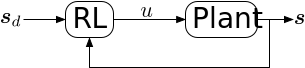
\includegraphics[width = 0.5\textwidth]{figures/figures_RL_model_based_control/Block_diagram_RL_alone.pdf}
\caption{Block diagram for Pure RL control structure} 
\label{fig_chap2:pure_RL_block_diagram}
\end{center}
\end{figure}
%

\subsection{RL and Fixed-Gain Control}
%
\begin{figure}[tb]
    \begin{center}
    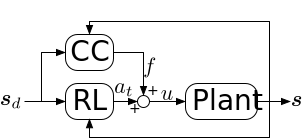
\includegraphics[width = 0.5\textwidth]{figures/figures_RL_model_based_control/Block_diagram_combined_control.pdf}
    \caption{Block diagram for RL and fixed-gain control structure} 
    \label{fig_chap2:fixed_gain_block_diagram}
    \end{center}
    \end{figure}
    %
    \begin{figure}[tb]
    \begin{center}
    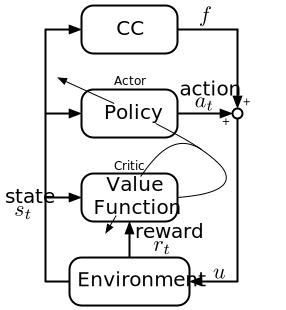
\includegraphics[width = 0.5\textwidth]{figures/figures_RL_model_based_control/Actor_Critic_diagram_fixed_gain.pdf}
    \caption{Learning diagram for RL with fixed-gain control} 
    \label{fig_chap2:fixed_gain_actor_critic}
    \end{center}
    \end{figure}
    %
One proposed control architecture for combining domain knowledge with RL uses fixed-gain control components in parallel with the learned policy. The block diagram for this control architecture is shown in Figure~\ref{fig_chap2:fixed_gain_block_diagram}, where the CC block represents Conventional Control, or a model-based controller designed using domain knowledge of dynamics and control. The plant input, $u$, for this control structure is:
%
\begin{equation}
u=f(\boldsymbol{s}) + a_t
\label{eq_chap2:fixed_RL_block_diagram}
\end{equation}
%
where $f(\boldsymbol{s})$ is a fixed-gain input that is a function of the state, $\boldsymbol{s}$.
The specific design of $f(\boldsymbol{s})$ depends on the system and goal of the controller.
%
For instance, it could be designed such that it could function on its own to provide satisfactory (though suboptimal) performance, or it can be designed to perform well for only a subset of the desired operation space for the system.

The RL component of the controller will still need to interact with the fixed-gain component and modify the controller output to optimize the combined control policy. This provides the designer with the ability to design a simple controller that can provide satisfactory performance while leaving the more difficult optimal control problem to be solved by the RL agent.
%
The training process for this type of controller is illustrated by a modified actor-critic training diagram in Figure~\ref{fig_chap2:fixed_gain_actor_critic}. The action output from the policy, $a_t$, is combined with the output from the conventional controller, $f$. The sum of the outputs, $u$, is the input to the environment.
% The output from the conventional controller and action from the policy combine to become the input for the environment.
However, the value function only evaluates the action, $a_t$, not the total input to the environment. Since the value function and policy are unaffected by the conventional control block, the addition of the fixed-gain term is equivalent to changing the environment.

\subsection{Agent-Driven Gain Scheduling}
%
\begin{figure}[tb]
\begin{center}
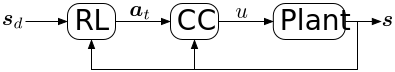
\includegraphics[width = 0.7\textwidth]{figures/figures_RL_model_based_control/Block_diagram_cont_gain_sched_control.pdf}
\caption{Block diagram for RL continuous gain-scheduling control structure} 
\label{fig_chap2:cont_gain_sched_block_diagram}
\end{center}
\end{figure}
%

In the fixed-gain and RL controller architecture, the agent is unable to modify the component of the controller designed using domain knowledge.
In addition to this controller architecture,
% using a fixed-gain controller in parallel with RL to take advantage of domain knowledge,
the combined controller can be designed to have the agent interact directly with the domain-knowledge controller. One way to realize this direct interaction is by using a gain-scheduled controller for which the agent learns the scheduling law. This is shown by the block diagram in Figure~\ref{fig_chap2:cont_gain_sched_block_diagram}, where the controller output, $u$, is:
% One of the control structures combining RL and controls domain knowledge is a agent-driven gain scheduling type of controller shown in the block diagram in Figure~\ref{fig_chap2:cont_gain_sched_block_diagram}.
% It can also be combined with a model-based fixed-gain term such that the plant input, $u$ from the controller is:
%
\begin{equation}
u = \boldsymbol{a}_t\boldsymbol{s}
\label{eq_chap2:cont_gain_sched_RL_block_diagram}
\end{equation}
%
and $\boldsymbol{a}_t$ is a vector of the agent outputs, $\boldsymbol{a}_t=[a_t^{(1)}, \, a_t^{(2)}, \, \dots, \, a_t^{(n)}]$, corresponding to a feedback controller with $n$ states.
Implementation of the agent as a gain scheduling mechanism allows for domain knowledge to be used to design the feedback controller.
It may also improve interpretability, since the response at each time step can be understood as a system subject to a linear feedback controller.
%
Figure~\ref{fig_chap2:gain_sched_actor_critic} shows the learning process for the gain-scheduled RL controller.
%
The set of actions, $a_t$, is a set of gains that are used to update the gain-scheduled feedback controller in the CC block. The output, $u$, from the controller is passed to the environment and causes its state, $s_t$, to change. The reward is used to update the value function so that the gain update law can be optimized. This controller architecture provides a more integrated combination between the parts of the controller designed using domain knowledge and the parts learned by RL.
%
\begin{figure}[tb]
    \begin{center}
    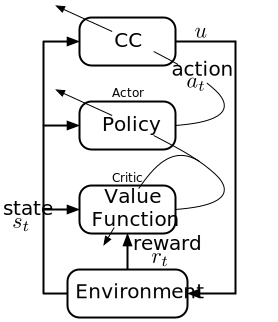
\includegraphics[width = 0.5\textwidth]{figures/figures_RL_model_based_control/Actor_Critic_diagram_gain_sched.pdf}
    \caption{Learning diagram for RL with gain scheduled control} 
    \label{fig_chap2:gain_sched_actor_critic}
    \end{center}
\end{figure}
%

Training RL agents requires selecting training parameters such as the RL algorithm, neural network architecture, and episode length. The training parameters were tuned for each benchmark problem and will be introduced for each system alongside each set of results. Additional information about the mechanical parameters for each benchmark system and the hyperparameters used for training are found in Appendix A.

\section{Duffing Oscillator Benchmark System}
\label{sec_chap2:Duffing_oscillator}
\subsection{Problem Description}

%
\begin{figure}[t]
\begin{center}
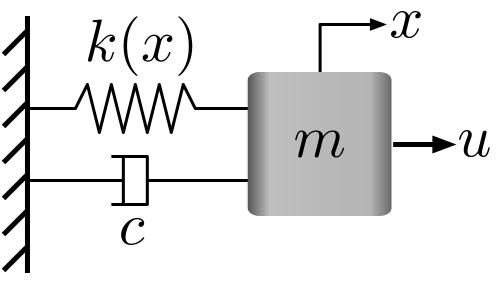
\includegraphics[width = 0.5\textwidth]{figures/figures_RL_model_based_control/Duffing_oscillator.pdf}
\caption{Duffing oscillator model}
\label{fig_chap2:duffing_model}
\end{center}
\end{figure}
% 
A duffing oscillator model was used as a simple benchmark model to illustrate the usefulness of combined RL and conventional control methods. The model is shown in Figure~\ref{fig_chap2:duffing_model}, where $m$ is the mass, $c$ is the damping coefficient, $x$ is the displacement, $k(x)$ is the nonlinear spring stiffness, and $u$ is the force input. The equation of motion for this system is:
%
\begin{equation}
m\ddot{x} + c\dot{x} + k(x)x = u
\label{eq_chap_2:duffing_EOM}
\end{equation}
%
where the nonlinear stiffness is
$k(x)=\alpha + \beta x^2$.
% $k(x)=\alpha + 3\beta x^2$.
The displacement is constrained between $-1.5\si{\meter}\leq x \leq 1.5\si{\meter}$. The desired behavior of the system is to move the mass from rest at $x=0$ to a desired displacement, $x_d$, while limiting oscillation amplitude. The reward function used to accomplish this was:
%
\begin{equation}
    r = -(x_d - x)^2
    \label{eq_chap2:duffing_reward_function}
\end{equation}
%
Although this reward function is simple, it accomplishes the desired task by requiring the position error to be quickly minimized in order to maximize reward.

The previously described combined control structures were applied to the duffing oscillator. The Pure RL controller uses a force output as the action applied to the system. For the combined controllers, a fixed-gain component was designed to provide a constant force that stabilizes the system about the desired displacement, $x_d$. The force which stabilizes the system at the desired equilibrium is:
%
\begin{equation}
f(\boldsymbol{s})=\alpha x_d + \beta x^3_d
\label{eq_chap_2:feedforward}
\end{equation}
%
% \rnotes{For the case with the fixed feedforward term alone (FF), the input allows the system to oscillate about the setpoint. Because of this, the controllers which combine the feedforward term and an agent in parallel, RL-LA and RL-PD, cause the system to nearly reach the setpoint. For these controllers, the model-based feedforward term is responsible for causing the system to perform the desired task of reaching the setpoint while the agent modifies the force input to reduce ISE.}
The response of the duffing oscillator with this fixed-gain controller and desired displacement of $x_d=1$ is shown in Figure~\ref{fig:duffing_feedforward}. Although the fixed-gain controller causes the system to move to the desired displacement, the settling time is high. In the combined controllers, the RL components are responsible for modifying the fixed-gain component to optimize the response.
%
\begin{figure}[tb]
    \centering
      % \vspace{-5ex}
      % \includegraphics[width=\columnwidth]{figures/RL_RL-PD_RL-LA_500steps}
      % \includegraphics[width=3in]{figures/RL_RL-PD_RL-LA_500steps}
      \includegraphics[width=0.65\columnwidth]{figures/figures_RL_model_based_control/time_responses_duffing/duffing_FF/Displacement_1_init_0_steps}
      \vspace{-2ex}
      \caption{Duffing oscillator response with fixed-gain term}
      % \vspace{-2ex}
      \label{fig:duffing_feedforward}
\end{figure}
%
This fixed-gain controller was used for two combined controllers, one that uses a single scalar action and another that uses a gain-scheduled controller. In summary, the set of controllers tested on the duffing oscillator are:
%
\begin{align}
    &\qquad\qquad\text{Pure RL:} & u&=a_t \qquad\qquad\qquad\\
    &\qquad\qquad\text{RL-PD:} & u&=\alpha x_d + \beta x_d^3 - a_t^{(1)}(x-x_d) - a_t^{(2)} \dot{x}\\
    &\qquad\qquad\text{RL-LA:} & u&=\alpha x_d + \beta x_d^3 + a_t \qquad\qquad\qquad
\end{align}
%
Pure RL is the baseline controller that uses the action, $a_t$, from RL as the only input to the system. RL-PD uses the fixed-gain controller in \eqref{eq_chap_2:feedforward} in addition to a Proportional-Derivative (PD) controller, where the actions $a_t^{(1)}$ and $a_t^{(2)}$ are gains for the displacement error and velocity of the system. RL-Lumped Action (RL-LA) uses the fixed-gain controller with a lumped action, or single scalar action. 

\subsection{Baseline Performance}
%
\begin{figure}[tb]
    \centering
      % \vspace{-5ex}
      % \includegraphics[width=\columnwidth]{figures/Duffing_ISE_while_training_shaded}
      % \includegraphics[width=3in]{figures/Duffing_ISE_while_training_shaded}
      \includegraphics[width=0.65\columnwidth]{figures/figures_RL_model_based_control/duffing_mean_reward_v_episode}
      \vspace{-2ex}
      \caption{Mean duffing oscillator reward during training}
      % \vspace{-2ex}
      \label{fig_chap2:duffing_reward_trend}
    \end{figure}
    %

The agents for each controller were trained using the Twin Delayed DDPG (TD3) algorithm~\cite{Fujimoto:2018a}.
%
All neural networks had two hidden layers, containing $400$ and $300$ nodes, respectively, and used the rectified linear unit (RELU) activation function as was used in the original TD3 paper. The observations included measurements of the displacement, $x$, and velocity, $\dot{x}$, of the mass, analogous to full-state feedback for a conventional controller, as well as the desired displacement, $x_d$.
%
Training was conducted over $40$ episodes.
% which is $80$ episodes at a $50\si{\hertz}$ sampling rate.
The desired displacement was randomized at the initialization of each episode.
% For each episode, a random setpoint is generated based on an initial seed.
Since RL relies on stochasticity, five agents were trained for each control structure. The same set of five initial seeds was used for the different control structures.
% After training was completed, a new trial begins with a new initial seed, and the agent is reinitialized. The same set of random seeds is used for each method. Fifteen trials were performed for each method.
%
After training the agents, they were tested to compare the performance of the controllers without model-based components to those with model-based and RL components.

%
The performance of the agents during training was evaluated at fixed intervals using the reward received from the system starting at rest with a desired displacement of $x_d=1\si{\meter}$.
The reward trends during training are shown in Figure~\ref{fig_chap2:duffing_reward_trend}, where the lines are the mean reward, and the shaded regions are standard deviation for the five agents of each controller type. The Pure RL controllers begin training with the lowest reward whereas the RL-PD controllers begin with the highest reward. Although the reward from the RL and RL-LA controllers tend to increase after the beginning of training, the reward from RL-PD initially significantly decreases. This is due to one of the responses becoming unstable, which skews the mean and standard deviation. The mean rewards from the different controllers converge to approximately the same value after 20 episodes.
%

Time responses from the agents at the beginning of training are shown in Figure~\ref{fig_chap2:duffing_0_steps}.
%
The low reward at the beginning of training with Pure RL was caused by one of the responses being unstable and the steady-state error from the other responses resulting from the inability of the controller to force the system to reach the desired displacement, $x_d$, as shown in Figure~\ref{subfig_chap2:duffing_pure_RL_0_steps}.
%
\begin{figure}[tb]
    \centering
    \begin{subfigure}[b]{0.49\textwidth}
        \centering
        \includegraphics[width=\textwidth]{figures/figures_RL_model_based_control/time_responses_duffing/duffing_pure_RL/Displacement_1_init_0_steps.pdf}
        \caption{Pure RL}
        \label{subfig_chap2:duffing_pure_RL_0_steps}
    \end{subfigure}\\
    \hfill
    \begin{subfigure}[b]{0.49\textwidth}
        \centering
        \includegraphics[width=\textwidth]{figures/figures_RL_model_based_control/time_responses_duffing/duffing_RL_PD/Displacement_1_init_0_steps.pdf}
        \caption{RL-PD}
        \label{subfig_chap2:duffing_RL_PD_0_steps}
    \end{subfigure}
    \hfill
    \begin{subfigure}[b]{0.49\textwidth}
        \centering
        \includegraphics[width=\textwidth]{figures/figures_RL_model_based_control/time_responses_duffing/duffing_RL_LA/Displacement_1_init_0_steps.pdf}
        \caption{RL-LA}
        \label{subfig_chap2:duffing_RL_LA_0_steps}
    \end{subfigure}
    \hfill
    \caption{Duffing oscillator responses before training}
    \label{fig_chap2:duffing_0_steps}
\end{figure}
%
% When using Pure RL, without a feedforward term, the agent does not cause the system to reach the desired setpoint.
%
Since the combined controllers have the fixed-gain component, \eqref{eq_chap_2:feedforward}, they cause the system to move near the desired displacement. The responses with RL-PD in Figure~\ref{subfig_chap2:duffing_RL_PD_0_steps} do not have overshoot and tend to have shorter settling times than the other controllers. Since the controller output of the gain-scheduled PD component is zero at the desired displacement, the combination of the fixed-gain component and PD component in RL-PD results in zero steady-state error. Similar to RL-PD, the RL-LA responses in Figure~\ref{subfig_chap2:duffing_RL_LA_0_steps} settle near the desired displacement. However, the responses have higher oscillation amplitude and some responses have steady-state error. These responses show that the combined controllers have better performance than the Pure RL controller even before training.
%

%
\begin{figure}[tb]
    \centering
    \begin{subfigure}[b]{0.49\textwidth}
        \centering
        \includegraphics[width=\textwidth]{figures/figures_RL_model_based_control/time_responses_duffing/duffing_pure_RL/Displacement_1_init_10000_steps.pdf}
        \caption{Pure RL}
        \label{subfig_chap2:duffing_pure_RL_10000_steps}
    \end{subfigure}\\
    \hfill
    \begin{subfigure}[b]{0.49\textwidth}
        \centering
        \includegraphics[width=\textwidth]{figures/figures_RL_model_based_control/time_responses_duffing/duffing_RL_PD/Displacement_1_init_10000_steps.pdf}
        \caption{RL-PD}
        \label{subfig_chap2:duffing_RL_PD_10000_steps}
    \end{subfigure}
    \hfill
    \begin{subfigure}[b]{0.49\textwidth}
        \centering
        \includegraphics[width=\textwidth]{figures/figures_RL_model_based_control/time_responses_duffing/duffing_RL_LA/Displacement_1_init_10000_steps.pdf}
        \caption{RL-LA}
        \label{subfig_chap2:duffing_RL_LA_10000_steps}
    \end{subfigure}
    \hfill
    \caption{Duffing oscillator responses after training}
    \label{fig_chap2:duffing_10000_steps}
\end{figure}
%
Time responses of the duffing oscillator after the agent controllers were trained are shown in Figure~\ref{fig_chap2:duffing_10000_steps}. The responses with Pure RL in Figure~\ref{subfig_chap2:duffing_pure_RL_10000_steps} settled near the desired displacement at $x_d=1\si{\meter}$ with low oscillation amplitude. However, all of the responses have steady-state error. The RL-PD responses in Figure~\ref{subfig_chap2:duffing_RL_PD_10000_steps} have zero steady-state error just as the responses before training. However, one response has overshoot and another response has a long rise time. The RL-LA responses in Figure~\ref{subfig_chap2:duffing_RL_LA_10000_steps} have short rise times; however, they have steady-state error and two of the responses have long settling times due to oscillation. The response characteristics of the Pure RL and combined controllers are summarized in Table~\ref{table:duffing_resp_char}. The RL-PD controllers had the best performance in all categories. Pure RL has higher mean steady-state error than RL-LA, however, RL-LA has much longer settling time and higher overshoot.
%
\begin{table}[tb]
    \begin{center}
      \setlength{\tabcolsep}{6pt}
      \caption{Duffing Oscillator Response Characteristics}
      \begin{tabular}{ l c c c c}
      \hline\hline
       & & Settling Time & Steady-state Error & Percent Overshoot \\
      \hline
      \multirow{2}{*}{\textbf{RL}} & \text{Mean} & 2.212\si{\second} & 0.064\si{\meter} & 6.047\%\\
       & \text{SD} & 2.885\si{\second} & 0.025\si{\meter} & 7.702\% \\
      \hline
      \multirow{2}{*}{\textbf{RL-PD}} & \text{Mean} & \textbf{1.372}\si{\second} & \textbf{0.0}\si{\meter} & \textbf{0.5}\%\\
       & \text{SD} & \textbf{0.598}\si{\second} & \textbf{0.0}\si{\meter} & \textbf{1.174}\%\\
      \hline
      \multirow{2}{*}{\textbf{RL-LA}} & \text{Mean} & 14.62\si{\second} & 0.0587\si{\meter} & 11.839\%\\
       & \text{SD} & 18.672\si{\second} & 0.0283\si{\meter} & 15.004\%\\
      \label{table:duffing_resp_char}
      \end{tabular}
      % \vspace{-0.2in}
    \end{center}
\end{table}
%

Although the Pure RL controller was not designed with any domain knowledge, it still provides good performance after training. RL-PD had the best performance overall. Its controller architecture also relied more heavily on domain knowledge since it included both a fixed-gain component and a state-feedback control component for which the agents only had to learn appropriate parameters. The responses from the RL-LA controllers have slightly lower steady-state error than the Pure RL controllers due to the fixed-gain component; however, settling times for RL-LA were inconsistent.
% more training would be required to get more consistent settling times. \dots

% \rnotes{Comment out overshoot and settling time plots during training.}
% \begin{figure}[tb]
% \centering
%   % \vspace{-5ex}
%   % \includegraphics[width=\columnwidth]{figures/RL_RL-PD_RL-LA_2500steps}
%   \includegraphics[width=0.65\columnwidth]{figures/figures_RL_model_based_control/RL_RL-PD_RL-LA_trial1_2500steps}
%   \vspace{-2ex}
%   \caption{Response at 2500 training steps}
%   % \vspace{-2ex}
%   \label{fig:Response_2500steps}
% \end{figure}
% %
% %
% \begin{figure}[tb]
% \centering
%   % \vspace{-5ex}
%   % \includegraphics[width=\columnwidth]{figures/RL_RL-PD_RL-LA_10000steps}
%   % \includegraphics[width=3in]{figures/RL_RL-PD_RL-LA_10000steps}
%   \includegraphics[width=0.65\columnwidth]{figures/figures_RL_model_based_control/RL_RL-PD_RL-LA_trial1_5000steps}
%   \vspace{-2ex}
%   \caption{Response at 5000 training steps}
%   % \vspace{-2ex}
%   \label{fig:Response_5000steps}
% \end{figure}
% %

% Although the reward used to train the agents is analogous to ISE, other performance metrics were also used to compare the performance of the combined feedforward and RL controllers to the controller using Pure RL. The mean $5\%$ settling times from the controllers during training are shown in Figure \ref{fig:Settingwhiletraining}. Due to the way settling time was measured, a settling time of $5\si{\second}$ in the figure corresponds to a true settling time of $5\si{\second}$ or longer.
% %
% The settling time with Pure RL remained above that of RL-PD and RL-LA throughout training. Although the settling time of RL-PD does not show a clear trend, the settling time for RL-LA tends to decrease as training progresses. The high settling times during training with RL and at the beginning of training with RL-LA primarily result from steady-state error, where the system settles at a position below the desired setpoint.

% The mean percent overshoot from the controllers, shown in Figure \ref{fig:Overshootwhiletraining}, was also used to evaluate the controllers. It follows a similar trend as was shown in the time response plots, where the overshoot from Pure RL at the beginning of training tends to be lower than that from RL-PD and RL-LA due to the system not reaching the desired setpoint. Although, the mean overshoot for the three methods are similar near the end of training, the mean maximum overshoot of Pure RL is significantly higher than that of the other methods.

% %
% \begin{figure}[tb]
% \centering
%   % \vspace{-5ex}
%   % \includegraphics[width=\columnwidth]{figures/Duffing_settling_while_training_shaded}
%   % \includegraphics[width=3in]{figures/Duffing_settling_while_training_shaded}
%   \includegraphics[width=0.65\columnwidth]{figures/figures_RL_model_based_control/Duffing_settling_while_training_mean}
%   \vspace{-2ex}
%   \caption{Mean settling time while training}
%   % \vspace{-2ex}
%   \label{fig:Settingwhiletraining}
% \end{figure}
% %
% \begin{figure}[tb]
% \centering
%   % \vspace{-5ex}
%   % \includegraphics[width=\columnwidth]{figures/Duffing_overshoot_while_training_shaded}
%   % \includegraphics[width=3in]{figures/Duffing_overshoot_while_training_shaded}
%   \includegraphics[width=0.65\columnwidth]{figures/figures_RL_model_based_control/Duffing_overshoot_while_training_mean}
%   \vspace{-2ex}
%   \caption{Mean percent overshoot while training}
%   % \vspace{-2ex}
%   \label{fig:Overshootwhiletraining}
% \end{figure}
% %

\section{Double-Pendulum Crane}
\subsection{Problem Description}
%
\begin{figure}[tb]
\begin{center}
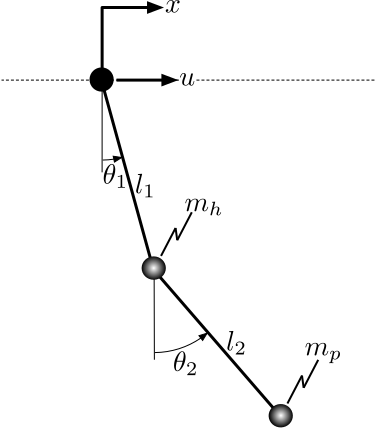
\includegraphics[width = 0.44\textwidth]{figures/figures_RL_model_based_control/Double_pendulum_crane_model.pdf}
\caption{Double-pendulum planar crane model}
\label{fig_chap2:planar_crane}
\end{center}
\end{figure}
%

A planar double-pendulum crane, shown by the model in Figure~\ref{fig_chap2:planar_crane}, was used as a second benchmark system for the combined RL controllers.
The double-pendulum crane is a three degree-of-freedom underactuated system.
This model approximates the dynamics of physical cranes where a payload is fastened to the crane by a hook with non-negligible mass. The payload is manipulated by moving a crane trolley on a horizontal track.
The displacement of the trolley along the track is described by $x$. The angular displacements of the hook and payload pendulums are $\theta_1$ and $\theta_2$, respectively, both measured from the vertical axis of the Newtonian frame. The lengths of the pendulums, commonly called hoist length and rigging length, are $l_1$ and $l_2$. The hook mass is $m_h$, and the payload mass is $m_p$. The input, $u$, is desired acceleration of the trolley. The goal of the controllers for this system was to move the trolley to a desired displacement while minimizing oscillation of the pendulums.
% \rph{Direct acceleration control was used as the system input, $u$.}
%
The equations of motion for the double-pendulum crane are:
%
% \begin{equation}
% \begin{multline}
% \dot{x},\\
% \dot{\theta_1},\\
% \dot{\theta_2},\\
% u_t,\\
% (-L_1*L2*mp*(sin(\theta_1)*sin(\theta_2) + cos(\theta_1)*cos(\theta_2))*(-L_1*L2*mp*(-sin(\theta_1)*cos(\theta_2) + sin(\theta_2)*cos(\theta_1))*\dot{\theta}_1^2 - L_1*L2*mp*(sin(\theta_1)*sin(\theta_2) + cos(\theta_1)*cos(\theta_2))*(-L_1*L2*mp*(sin(\theta_1)*cos(\theta_2) - sin(\theta_2)*cos(\theta_1))*\dot{\theta_2}^2 - L_1*g*mh*sin(\theta_1) - L_1*g*mp*sin(\theta_1))/(L_1^2*mh + L_1^2*mp) - L2*g*mp*sin(\theta_2) - (-L_1*L2*mp*(sin(\theta_1)*sin(\theta_2) + cos(\theta_1)*cos(\theta_2))*(L_1*mh*cos(\theta_1) + L_1*mp*cos(\theta_1))/(L_1^2*mh + L_1^2*mp) + L2*mp*cos(\theta_2))*acceleration_command)/(-L_1^2*L2^2*mp^2*(sin(\theta_1)*sin(\theta_2) + cos(\theta_1)*cos(\theta_2))^2/(L_1^2*mh + L_1^2*mp) + L2^2*mp) - L_1*L2*mp*(sin(\theta_1)*cos(\theta_2) - sin(\theta_2)*cos(\theta_1))*\dot{\theta_2}^2 - L_1*g*mh*sin(\theta_1) - L_1*g*mp*sin(\theta_1) - (L_1*mh*cos(\theta_1) + L_1*mp*cos(\theta_1))*acceleration_command)/(L_1^2*mh + L_1^2*mp),\\
% (-L_1*L2*mp*(-sin(\theta_1)*cos(\theta_2) + sin(\theta_2)*cos(\theta_1))*\dot{\theta_1}^2 - L_1*L2*mp*(sin(\theta_1)*sin(\theta_2) + cos(\theta_1)*cos(\theta_2))*(-L_1*L2*mp*(sin(\theta_1)*cos(\theta_2) - sin(\theta_2)*cos(\theta_1))*\dot{\theta_2}^2 - L_1*g*mh*sin(\theta_1) - L_1*g*mp*sin(\theta_1))/(L_1^2*mh + L_1^2*mp) - L2*g*mp*sin(\theta_2) - (-L_1*L2*mp*(sin(\theta_1)*sin(\theta_2) + cos(\theta_1)*cos(\theta_2))*(L_1*mh*cos(\theta_1) + L_1*mp*cos(\theta_1))/(L_1^2*mh + L_1^2*mp) + L2*mp*cos(\theta_2))*acceleration_command)/(-L_1^2*L2^2*mp^2*(sin(\theta_1)*sin(\theta_2) + cos(\theta_1)*cos(\theta_2))^2/(L_1^2*mh + L_1^2*mp) + L2^2*mp)
% \end{multline}
% \end{equation}
%
\begin{multline}
\left [
\begin{array}{ccc}
1 & 0 & 0\\
l_1\cos(\theta_1)(m_h + m_p) & l_1^2(m_h + m_p) & l_1l_2m_p\cos(\theta_1-\theta_2)\\
l_2m_p\cos(\theta_2) & l_1l_2m_p\cos{(\theta_1-\theta_2)} & l_2^2m_p\\
\end{array}
\right ]
\left [
\begin{array}{c}
\ddot{x}\\
\ddot{\theta}_1\\
\ddot{\theta}_2
\end{array}
\right ] \\
=
\left [
\begin{array}{c}
u\\
-l_1l_2m_p\sin(\theta_1-\theta_2)\dot{\theta}_2^2 - l_1g\sin(\theta_1)(m_h + m_p)\\
-l_1l_2m_p\sin(\theta_2-\theta_1)\dot{\theta}_1^2 - l_2gm_p\sin(\theta_2)\\
\end{array}
\right ]
\end{multline}
%
The acceleration of the crane trolley, $\ddot{x}$, is determined by only the control output, $u$. The dynamics of the pendulums are coupled with each other and the acceleration of the trolley.
%
The incremental reward function for this system is:
%
\begin{equation}
r = -\omega_xx^2 - \omega_{\theta_1}\theta_1^2 - \omega_{\theta_2}\theta_2^2
\label{eq_chap2:reward_crane}
\end{equation}
%
where $\omega_x$, $\omega_{\theta_1}$, and $\omega_{\theta_2}$ are weights designed to normalize the reward terms to have approximately equal importance during training.

%
\begin{figure}[tb]
    \centering
    \begin{subfigure}[b]{0.49\textwidth}
        \centering
        \includegraphics[width=\textwidth]{figures/figures_RL_model_based_control/time_responses_crane/dpcrane_fixed_gain/Cart_displacement_0p185_init_300000_steps.pdf}
        \caption{Trolley displacement response}
        \label{subfig_chap2:dpcrane_fixed_gain_trolley_resp}
    \end{subfigure}\\
    \hfill
    \begin{subfigure}[b]{0.49\textwidth}
        \centering
        \includegraphics[width=\textwidth]{figures/figures_RL_model_based_control/time_responses_crane/dpcrane_fixed_gain/Hook_displacement_0p185_init_300000_steps.pdf}
        \caption{Hook displacement response}
        \label{subfig_chap2:dpcrane_fixed_gain_hook_resp}
    \end{subfigure}
    \hfill
    \begin{subfigure}[b]{0.49\textwidth}
        \centering
        \includegraphics[width=\textwidth]{figures/figures_RL_model_based_control/time_responses_crane/dpcrane_fixed_gain/Payload_displacement_0p185_init_300000_steps.pdf}
        \caption{Payload displacement response}
        \label{subfig_chap2:dpcrane_fixed_gain_payload_resp}
    \end{subfigure}
    \hfill
    \caption{Crane responses from fixed-gain term}
    \label{fig_chap2:dpcrane_fixed_gain_resp}
\end{figure}
%

The Pure RL, fixed-gain and RL, and gain-scheduled RL control elements were applied to this system. The fixed-gain term, $f(\boldsymbol{s})=k_p x + k_d \dot{x}$, is a PD controller, where the gains, $k_p$ and $k_d$, are designed to move the trolley to the desired displacement without input saturation and with a damping coefficient of $\zeta=\frac{\sqrt{2}}{2}$.
%
Time responses of the crane subject to the fixed-gain controller are shown in Figure~\ref{fig_chap2:dpcrane_fixed_gain_resp}. This movement excites unwanted oscillation in the pendulums, shown in Figure~\ref{subfig_chap2:dpcrane_fixed_gain_hook_resp} and Figure~\ref{subfig_chap2:dpcrane_fixed_gain_payload_resp}. Since the fixed-gain controller does not account for motion of the pendulums, the agent must modify the control output to limit hook and payload oscillation.
%

Multiple combined controllers consisting of fixed-gain, gain-scheduled, and lumped action terms were tested on the benchmark double-pendulum crane.
%
While the fixed-gain term only accounts for the trolley position and velocity, the gain scheduling term only accounts for pendulum motion. Because of this, one combined controller uses the fixed-gain control element combined with the gain-scheduled control element. Another combined controller uses the fixed-gain terms with a lumped action term learned by the agent.
Additionally, a controller combining the features of all the above controllers was tested, where the control output is determined by a fixed-gain, gain-scheduled, and lumped-action control elements. In summary, the control laws for the crane are:
%
\begin{align}
&\qquad\qquad\text{Pure RL:} & u&=a_t \qquad\qquad\qquad\\
&\qquad\qquad\text{RL-PD:} & u&=k_px+k_d\dot{x} + \boldsymbol{a}_t\boldsymbol{\theta} \qquad\qquad\qquad\\
&\qquad\qquad\text{RL-LA:} & u&=k_px+k_d\dot{x} + a_t \qquad\qquad\qquad\\
&\qquad\qquad\text{RL-PD-LA:} & u&=k_px+k_d\dot{x} + \boldsymbol{a}_t\boldsymbol{\theta} + a_t \qquad\qquad\qquad
\end{align}
%
where Pure RL is the baseline RL controller that does not utilize any domain knowledge. RL-PD is the controller with the fixed-gain term combined with a gain-scheduled term, where $\boldsymbol{a}_t$ are gains assigned by the agent and are updated at every time step, and $\boldsymbol{\theta}$ are the states describing the motion of the pendulums. RL-Lumped-Action (RL-LA) uses the fixed-gain control element with a single (lumped) action from the agent. RL-PD-LA combines fixed-gain, gain-scheduled, and lumped action control elements.
% where $\boldsymbol{a}_t$ are the agent assigned gains for the pendulum states and $\boldsymbol{\theta}$ is the vector of angular states. \rnotes{Maybe I could use a different symbol.}

\subsection{Baseline Performance}
%
\begin{figure}[tb]
        \centering
        \includegraphics[width=0.65\columnwidth]{figures/figures_RL_model_based_control/dpcrane_mean_reward_v_episode.pdf}
        \vspace{-2ex}
        \caption{Mean crane reward during training for $x(0)=0.185\si{\meter}$}
      % \vspace{-2ex}
        \label{fig:dpcrane_mean_reward_baseline}
\end{figure}
%
The TD3 algorithm~\cite{Fujimoto:2018a} was used to train five agents for each controller using Pure RL, RL-PD, RL-LA, and RL-PD-LA. The same set of five initial seeds was used for the different controllers. Each episode during training was initialized with the crane at rest with a trolley displacement of $x(0)=0.185\si{\meter}$ and hook and payload angular displacements of $\theta_1=\theta_2=0$. The desired final displacement of the trolley was $x(t_f)=0\si{\meter}$. Trends during training are shown to evaluate the baseline performance of the controller types. Figure \ref{fig:dpcrane_mean_reward_baseline} shows the mean reward earned from the five trained agents of each controller type. The shaded region shows the standard deviation of the rewards at each sampled episode of training. The untrained performance of the combined controllers at 0 episodes is better than that of the controller using Pure RL. However, near the end of training, at 3000 episodes, the rewards earned by each controller are approximately equal.
%

The higher initial reward from the combined controllers is due to the fixed-gain term commanding the trolley to move to the desired location, whereas more training is necessary for the agent of the Pure RL controller to learn to move the trolley to the desired location.
%
This can be seen by isolating the contribution of the trolley response to the total reward, where the reward contribution from the trolley is:
%
\begin{equation}
    r_{x} = -\omega_x x^2
\end{equation}
%
The reward from the trolley is shown in Figure~\ref{fig:mean_settling_baseline}.
%
Although the combined controllers start with higher reward from the trolley displacement, the agents for the Pure RL controller learn to increase the trolley reward after training for only a short time. The trolley reward for RL-LA tends to be the highest for the controllers tested.
%
\begin{figure}[tb]
    \centering
    % \includegraphics[width=\columnwidth]{figures/Mean_settling_v_episode.pdf}
    \includegraphics[width=0.65\columnwidth]{figures/figures_RL_model_based_control/Trolley_reward_v_episode.pdf}
    \vspace{-2ex}
    % \caption{Mean settling time during training}
    \caption{Mean reward from trolley during training}
  % \vspace{-2ex}
    \label{fig:mean_settling_baseline}
\end{figure}
  %

Figure~\ref{fig_chap2:dpcrane_trolley_resp_0steps} shows the trolley displacement responses for the different controllers before training.
% where the neural network parameters of the agents are randomly initialized.
The crane begins at rest with initial trolley displacement of $x(0)=0.185\si{\meter}$ and pendulum displacements $\theta_1=\theta_2=0$.
The trolley responses for Pure RL do not settle near the equilibrium and instead diverge towards the limits of the workspace, as shown in Figure~\ref{subfig_chap2:dpcrane_trolley_resp_0steps_pure_RL}. The responses for RL-PD in Figure~\ref{subfig_chap2:dpcrane_trolley_resp_0steps_gain_sched} have the best trolley performance, where most of the responses converge near the desired displacement with low oscillation amplitude due to the fixed-gain terms. The RL-LA responses in Figure~\ref{subfig_chap2:dpcrane_trolley_resp_0steps_RL_LA} have higher error in trolley displacement than RL-PD but have lower oscillation amplitude. The RL-PD-LA responses in Figure~\ref{subfig_chap2:dpcrane_trolley_resp_0steps_RL_PD_LA} have less trolley displacement error than RL-LA, but some of the responses have high oscillation amplitude.
%
\begin{figure}[tb]
    \centering
    \begin{subfigure}[b]{0.49\textwidth}
        \centering
        \includegraphics[width=\textwidth]{figures/figures_RL_model_based_control/time_responses_crane/dpcrane_pure_RL/Cart_displacement_0p185_init_0_steps.pdf}
        \caption{Pure RL}
        \label{subfig_chap2:dpcrane_trolley_resp_0steps_pure_RL}
    \end{subfigure}
    \hfill
    \begin{subfigure}[b]{0.49\textwidth}
	    \centering
	    \includegraphics[width=\textwidth]{figures/figures_RL_model_based_control/time_responses_crane/dpcrane_cont_gain_sched/Cart_displacement_0p185_init_0_steps.pdf}
	    \caption{RL-PD}
	    \label{subfig_chap2:dpcrane_trolley_resp_0steps_gain_sched}
    \end{subfigure}
    \hfill
    \begin{subfigure}[b]{0.49\textwidth}
        \centering
        \includegraphics[width=\textwidth]{figures/figures_RL_model_based_control/time_responses_crane/dpcrane_RL_LA/Cart_displacement_0p185_init_0_steps.pdf}
        \caption{RL-LA}
        \label{subfig_chap2:dpcrane_trolley_resp_0steps_RL_LA}
    \end{subfigure}
    \hfill
    \begin{subfigure}[b]{0.49\textwidth}
        \centering
        \includegraphics[width=\textwidth]{figures/figures_RL_model_based_control/time_responses_crane/dpcrane_RL_PD_LA/Cart_displacement_0p185_init_0_steps.pdf}
        \caption{RL-PD-LA}
        \label{subfig_chap2:dpcrane_trolley_resp_0steps_RL_PD_LA}
    \end{subfigure}
    \hfill
    \caption{Crane trolley responses for $x(0)=0.185\si{\meter}$ before training}
    \label{fig_chap2:dpcrane_trolley_resp_0steps}
\end{figure}
%

Figure~\ref{fig_chap2:dpcrane_trolley_resp_300000steps} shows the trolley displacement responses for the different controllers after training, where the crane begins at rest with initial trolley displacement of $x(0)=0.185\si{\meter}$ and pendulum displacements $\theta_1=\theta_2=0$.
Three of the five Pure RL agents shown in Figure~\ref{subfig_chap2:dpcrane_trolley_resp_300000steps_pure_RL} can bring the trolley to the desired displacement within the allotted time, whereas two responses do not converge to zero displacement. The RL-PD responses in Figure~\ref{subfig_chap2:dpcrane_trolley_resp_300000steps_gain_sched} tend to have higher oscillation amplitude than the other controllers. Figure~\ref{subfig_chap2:dpcrane_trolley_resp_300000steps_RL_LA} shows that the RL-LA responses tend to be able to converge closer to zero displacement than Pure RL. The RL-PD-LA responses in Figure~\ref{subfig_chap2:dpcrane_trolley_resp_300000steps_RL_PD_LA} are also able to converge to be close to the desired displacement at $x(t_f)=0\si{\meter}$, but exhibit some oscillation.
%
\begin{figure}[tb]
    \centering
    \begin{subfigure}[b]{0.49\textwidth}
        \centering
        \includegraphics[width=\textwidth]{figures/figures_RL_model_based_control/time_responses_crane/dpcrane_pure_RL/Cart_displacement_0p185_init_300000_steps.pdf}
        \caption{Pure RL}
        \label{subfig_chap2:dpcrane_trolley_resp_300000steps_pure_RL}
    \end{subfigure}
    \hfill
    \begin{subfigure}[b]{0.49\textwidth}
	    \centering
	    \includegraphics[width=\textwidth]{figures/figures_RL_model_based_control/time_responses_crane/dpcrane_cont_gain_sched/Cart_displacement_0p185_init_300000_steps.pdf}
	    \caption{RL-PD}
	    \label{subfig_chap2:dpcrane_trolley_resp_300000steps_gain_sched}
    \end{subfigure}
    \hfill
    \begin{subfigure}[b]{0.49\textwidth}
        \centering
        \includegraphics[width=\textwidth]{figures/figures_RL_model_based_control/time_responses_crane/dpcrane_RL_LA/Cart_displacement_0p185_init_300000_steps.pdf}
        \caption{RL-LA}
        \label{subfig_chap2:dpcrane_trolley_resp_300000steps_RL_LA}
    \end{subfigure}
    \hfill
    \begin{subfigure}[b]{0.49\textwidth}
        \centering
        \includegraphics[width=\textwidth]{figures/figures_RL_model_based_control/time_responses_crane/dpcrane_RL_PD_LA/Cart_displacement_0p185_init_300000_steps.pdf}
        \caption{RL-PD-LA}
        \label{subfig_chap2:dpcrane_trolley_resp_300000steps_RL_PD_LA}
    \end{subfigure}
    \hfill
    \caption{Crane trolley responses for $x(0)=0.185\si{\meter}$ after training}
    \label{fig_chap2:dpcrane_trolley_resp_300000steps}
\end{figure}
%
In both the cases before training and after training, the controllers utilizing a continuous gain scheduled term, RL-PD and RL-PD-LA, tend to exhibit oscillation near the desired displacement, whereas the controllers using a lumped action, Pure RL and RL-LA, have much lower oscillation amplitude. For the responses after training, the controllers that include a fixed-gain term and a lumped action, RL-LA and RL-PD-LA, tend to converge closer to the desired equilibrium and have lower steady state-error.
%
The response characteristics of the trolley are summarized in Table~\ref{table:dpcrane_trolley_resp_char}. RL-LA has the lowest values for all of the performance metrics shown. Although RL-PD has lower steady-state error and overshoot than Pure RL, it has higher residual oscillation amplitude. RL-PD-LA has lower steady-state error than Pure RL, but has higher values for residual oscillation amplitude and overshoot. In general, the combined controllers tend to have better performance than Pure RL for steady-state error and percent overshoot. However, RL-PD and RL-PD-LA have higher residual oscillation amplitudes due to the gain scheduling terms on the pendulum states.
%
\begin{table}[tb]
    \begin{center}
      \setlength{\tabcolsep}{6pt}
      \caption{Trolley Response Characteristics for $x(0)=0.185\si{\meter}$}
      \begin{tabular}{ l c c c c}
      \hline\hline
       & & Amplitude & Steady-state Error & Percent Overshoot \\
      \hline
      \multirow{2}{*}{\textbf{RL}} & \text{Mean} & 0.0005\si{\meter} & 0.027\si{\meter} & 24.8\%\\
       & \text{SD} & 0.0007\si{\meter} & 0.025\si{\meter} & 18.5\% \\
      \hline
      \multirow{2}{*}{\textbf{RL-PD}} & \text{Mean} & 0.004\si{\meter} & 0.024\si{\meter} & 21.6\%\\
       & \text{SD} & 0.003\si{\meter} & 0.017\si{\meter} & 17.4\%\\
      \hline
      \multirow{2}{*}{\textbf{RL-LA}} & \text{Mean} & \textbf{0.0}\si{\meter} & \textbf{0.02}\si{\meter} & \textbf{13.9}\%\\
       & \text{SD} & \textbf{0.0}\si{\meter} & \textbf{0.014}\si{\meter} & \textbf{5.9}\%\\
      \hline
      \multirow{2}{*}{\textbf{RL-PD-LA}} & \text{Mean} & 0.007\si{\meter} & 0.024\si{\meter} & 28.2\%\\
       & \text{SD} & 0.01\si{\meter} & 0.029\si{\meter} & 34\%\\
      \label{table:dpcrane_trolley_resp_char}
      \end{tabular}
      % \vspace{-0.2in}
    \end{center}
\end{table}
%

%
\begin{figure}[tb]
    \centering
    % \includegraphics[width=\columnwidth]{figures/Mean_swing_ISE_v_episode.pdf}
    \includegraphics[width=0.65\columnwidth]{figures/figures_RL_model_based_control/Swing_reward_v_episode.pdf}
    \vspace{-2ex}
    % \caption{Mean ISE of hook and payload swing during training}
    \caption{Mean reward from hook and payload during training}
  % \vspace{-2ex}
    \label{fig:mean_swing_ISE_baseline}
\end{figure}
%
% The mean reward shown in Figure~\ref{fig:dpcrane_mean_reward_baseline} also showed that RL-LA began training with the highest overall reward.
%
The previous evaluation of the contribution of the trolley responses to the reward is not adequate to understand the performance of the agents. Therefore, the reward contribution from the pendulum responses also needs to be analyzed.
% Since the contribution of the trolley response to total reward was analyzed in the previous paragraphs, the contribution of the pendulum responses needs to be analyzed as well.
% \rph{Since the fixed-gain term of the combined controllers was shown to provide similar trolley rewards, the difference in overall reward at training initialization is due to pendulum oscillation.}
The reward contribution from the oscillation of the hook and payload is:
%
\begin{equation}
    r_{\theta_1,\theta_2}=-\omega_{\theta_1} \theta_1^2 - \omega_{\theta_2} \theta_2^2
\end{equation}
%
The reward trends from the pendulum contributions are shown in Figure~\ref{fig:mean_swing_ISE_baseline}.
%
At the initialization of training, Pure RL begins with the highest reward followed by RL-LA with a slightly lower reward. The RL-PD and RL-PD-LA controllers have the lowest swing angle reward.
%
%
\begin{figure}[tb]
    \centering
    \begin{subfigure}[b]{0.49\textwidth}
        \centering
        \includegraphics[width=\textwidth]{figures/figures_RL_model_based_control/time_responses_crane/dpcrane_pure_RL/Payload_displacement_0p185_init_0_steps.pdf}
        \caption{Pure RL}
        \label{subfig_chap2:dpcrane_payload_resp_0steps_pure_RL}
    \end{subfigure}
    \hfill
    \begin{subfigure}[b]{0.49\textwidth}
	    \centering
	    \includegraphics[width=\textwidth]{figures/figures_RL_model_based_control/time_responses_crane/dpcrane_cont_gain_sched/Payload_displacement_0p185_init_0_steps.pdf}
	    \caption{RL-PD}
	    \label{subfig_chap2:dpcrane_payload_resp_0steps_gain_sched}
    \end{subfigure}
    \hfill
    \begin{subfigure}[b]{0.49\textwidth}
        \centering
        \includegraphics[width=\textwidth]{figures/figures_RL_model_based_control/time_responses_crane/dpcrane_RL_LA/Payload_displacement_0p185_init_0_steps.pdf}
        \caption{RL-LA}
        \label{subfig_chap2:dpcrane_payload_resp_0steps_RL_LA}
    \end{subfigure}
    \hfill
    \begin{subfigure}[b]{0.49\textwidth}
        \centering
        \includegraphics[width=\textwidth]{figures/figures_RL_model_based_control/time_responses_crane/dpcrane_RL_PD_LA/Payload_displacement_0p185_init_0_steps.pdf}
        \caption{RL-PD-LA}
        \label{subfig_chap2:dpcrane_payload_resp_0steps_RL_PD_LA}
    \end{subfigure}
    \hfill
    \caption{Crane payload responses for $x(0)=0.185\si{\meter}$ before training}
    \label{fig_chap2:dpcrane_payload_resp_0steps}
\end{figure}
%
The time responses of the payload before training are shown in Figure~\ref{fig_chap2:dpcrane_payload_resp_0steps}. The crane began at rest with an initial trolley displacement of $x(0)=0.185\si{\meter}$. The responses with Pure RL in Figure~\ref{subfig_chap2:dpcrane_payload_resp_0steps_pure_RL} and RL-LA in Figure~\ref{subfig_chap2:dpcrane_payload_resp_0steps_RL_LA} have relatively low oscillation amplitude. The RL-PD responses in Figure~\ref{subfig_chap2:dpcrane_payload_resp_0steps_gain_sched} and RL-PD-LA responses in Figure~\ref{subfig_chap2:dpcrane_payload_resp_0steps_RL_PD_LA} have higher amplitude oscillation, with some responses increasing amplitude with time. This corresponds with what was seen for the trolley responses at the start of training, where the controllers using agent-driven gain scheduling tended to have higher oscillation amplitude.

Figure~\ref{fig_chap2:dpcrane_payload_resp_300000steps} shows the time responses of the payload after training has been completed. The controllers that include a single lumped action term tend to have lower oscillation amplitude. This can be seen for Pure RL in Figure~\ref{subfig_chap2:dpcrane_payload_resp_300000steps_pure_RL}, RL-LA in Figure~\ref{subfig_chap2:dpcrane_payload_resp_300000steps_RL_LA} and RL-PD-LA in Figure~\ref{subfig_chap2:dpcrane_payload_resp_300000steps_RL_PD_LA}. RL-LA has the lowest oscillation amplitude, whereas RL-PD in Figure~\ref{subfig_chap2:dpcrane_payload_resp_300000steps_gain_sched} has the highest oscillation amplitude. This is consistent with the previous figures showing that the controllers that include a gain scheduling term tend to have higher oscillation amplitude. This is summarized in Table~\ref{table:dpcrane_payload_resp_char}, where RL-LA had the lowest mean residual oscillation amplitude. Although the mean oscillation amplitude for RL-PD-LA is the second highest, this was primarily due to one response skewing the mean.
%
\begin{figure}[tb]
    \centering
    \begin{subfigure}[b]{0.49\textwidth}
        \centering
        \includegraphics[width=\textwidth]{figures/figures_RL_model_based_control/time_responses_crane/dpcrane_pure_RL/Payload_displacement_0p185_init_300000_steps.pdf}
        \caption{Pure RL}
        \label{subfig_chap2:dpcrane_payload_resp_300000steps_pure_RL}
    \end{subfigure}
    \hfill
    \begin{subfigure}[b]{0.49\textwidth}
	    \centering
	    \includegraphics[width=\textwidth]{figures/figures_RL_model_based_control/time_responses_crane/dpcrane_cont_gain_sched/Payload_displacement_0p185_init_300000_steps.pdf}
	    \caption{RL-PD}
	    \label{subfig_chap2:dpcrane_payload_resp_300000steps_gain_sched}
    \end{subfigure}
    \hfill
    \begin{subfigure}[b]{0.49\textwidth}
        \centering
        \includegraphics[width=\textwidth]{figures/figures_RL_model_based_control/time_responses_crane/dpcrane_RL_LA/Payload_displacement_0p185_init_300000_steps.pdf}
        \caption{RL-LA}
        \label{subfig_chap2:dpcrane_payload_resp_300000steps_RL_LA}
    \end{subfigure}
    \hfill
    \begin{subfigure}[b]{0.49\textwidth}
        \centering
        \includegraphics[width=\textwidth]{figures/figures_RL_model_based_control/time_responses_crane/dpcrane_RL_PD_LA/Payload_displacement_0p185_init_300000_steps.pdf}
        \caption{RL-PD-LA}
        \label{subfig_chap2:dpcrane_payload_resp_300000steps_RL_PD_LA}
    \end{subfigure}
    \hfill
    \caption{Crane payload responses for $x(0)=0.185\si{\meter}$ after training}
    \label{fig_chap2:dpcrane_payload_resp_300000steps}
\end{figure}
%
%
\begin{table}[tb]
    \begin{center}
      \setlength{\tabcolsep}{6pt}
      \caption{Payload Residual Amplitude for $x(0)=0.185\si{\meter}$}
      \begin{tabular}{ l c c }
      \hline\hline
       & & Amplitude \\
      \hline
      \multirow{2}{*}{\textbf{RL}} & \text{Mean} & 0.474$^\circ$ \\
       & \text{SD} & 0.481$^\circ$ \\
      \hline
      \multirow{2}{*}{\textbf{RL-PD}} & \text{Mean} & 0.896$^\circ$ \\
       & \text{SD} & 0.23$^\circ$ \\
      \hline
      \multirow{2}{*}{\textbf{RL-LA}} & \text{Mean} & \textbf{0.015}$^\circ$ \\
       & \text{SD} & \textbf{0.03}$^\circ$ \\
      \hline
      \multirow{2}{*}{\textbf{RL-PD-LA}} & \text{Mean} & 0.756$^\circ$\\
       & \text{SD} & 0.947$^\circ$ \\
      \label{table:dpcrane_payload_resp_char}
      \end{tabular}
      % \vspace{-0.2in}
    \end{center}
\end{table}

The RL-LA controllers and RL-PD-LA controllers have the best overall performance in terms of limiting steady-state error and oscillation amplitude. They both tend to have lower trolley displacement error, where RL-PD-LA has lower error than RL-LA. However, RL-PD-LA achieves lower trolley steady-state error at the expense of higher pendulum oscillation. The Pure RL controllers tend to have the most trolley steady-state error since they do not have the benefit of the fixed-gain term to move the trolley towards zero displacement.

The results for the double-pendulum crane shown above were acquired from responses with initial trolley displacements equal to the one used for training. The fixed initial displacement of $x(0)=0.185\si{\meter}$ during training caused the agents to have the most experience for trolley displacements $0\leq x\leq 0.185\si{\meter}$. To show how the agents perform for initial displacements other than the one used for training, the following results show how the agents that were trained with an initial displacement of $x(0)=0.185\si{\meter}$ perform for an initial trolley displacement of $x(0)=-0.185\si{\meter}$ instead.
%
The reward trends from this initial trolley displacement are shown in Figure~\ref{fig:dpcrane_neg_mean_reward_baseline}. The initial rewards at the beginning of training are similar to those for initial displacements of $x(0)=0.185\si{\meter}$ in Figure~\ref{fig:dpcrane_mean_reward_baseline}. The fixed-gain terms cause the rewards from the combined controllers to begin higher than that of Pure RL. However, while the performance of the Pure RL controllers showed improvement from the initial reward, the other controllers do not show clear trends in improved performance.

%
\begin{figure}[tb]
    \centering
    \includegraphics[width=0.65\columnwidth]{figures/figures_RL_model_based_control/dpcrane_neg_mean_reward_v_episode.pdf}
    \vspace{-2ex}
    \caption{Mean crane reward during training for $x(0)=-0.185\si{\meter}$}
  % \vspace{-2ex}
    \label{fig:dpcrane_neg_mean_reward_baseline}
\end{figure}
%
\begin{figure}[h!]
    \centering
    \begin{subfigure}[b]{0.49\textwidth}
        \centering
        \includegraphics[width=\textwidth]{figures/figures_RL_model_based_control/time_responses_crane/dpcrane_pure_RL/Cart_displacement_-0p185_init_300000_steps.pdf}
        \caption{Pure RL}
        \label{subfig_chap2:dpcrane_neg_trolley_resp_300000steps_pure_RL}
    \end{subfigure}
    \hfill
    \begin{subfigure}[b]{0.49\textwidth}
	    \centering
	    \includegraphics[width=\textwidth]{figures/figures_RL_model_based_control/time_responses_crane/dpcrane_cont_gain_sched/Cart_displacement_-0p185_init_300000_steps.pdf}
	    \caption{RL-PD}
	    \label{subfig_chap2:dpcrane_neg_trolley_resp_300000steps_gain_sched}
    \end{subfigure}
    \hfill
    \begin{subfigure}[b]{0.49\textwidth}
        \centering
        \includegraphics[width=\textwidth]{figures/figures_RL_model_based_control/time_responses_crane/dpcrane_RL_LA/Cart_displacement_-0p185_init_300000_steps.pdf}
        \caption{RL-LA}
        \label{subfig_chap2:dpcrane_neg_trolley_resp_300000steps_RL_LA}
    \end{subfigure}
    \hfill
    \begin{subfigure}[b]{0.49\textwidth}
        \centering
        \includegraphics[width=\textwidth]{figures/figures_RL_model_based_control/time_responses_crane/dpcrane_RL_PD_LA/Cart_displacement_-0p185_init_300000_steps.pdf}
        \caption{RL-PD-LA}
        \label{subfig_chap2:dpcrane_neg_trolley_resp_300000steps_RL_PD_LA}
    \end{subfigure}
    \hfill
    \caption{Crane trolley responses for $x(0)=-0.185\si{\meter}$ after training}
    \label{fig_chap2:dpcrane_neg_trolley_resp_300000steps}
\end{figure}
%
Figure~\ref{fig_chap2:dpcrane_neg_trolley_resp_300000steps} shows the trolley response from $x(0)=-0.185\si{\meter}$ for the agents trained from $x(0)=0.185\si{\meter}$. Two responses with the Pure RL controller in Figure~\ref{subfig_chap2:dpcrane_neg_trolley_resp_300000steps_pure_RL} converge quickly towards the desired displacement at $x(t_f)=0\si{\meter}$; however, three responses converge slowly. Although the agents have no experience starting from this initial displacement, the combined controller responses tend to have lower trolley error due to the contribution from the fixed-gain terms. Several of the RL-PD responses in Figure~\ref{subfig_chap2:dpcrane_neg_trolley_resp_300000steps_gain_sched} quickly converge towards the desired displacement, but two responses move away from it again. Three of the RL-LA responses in Figure~\ref{subfig_chap2:dpcrane_neg_trolley_resp_300000steps_RL_LA} converge to be near the desired displacement; however, two of the responses stay near the initial displacement. Similarly, most of the RL-PD-LA responses in Figure~\ref{subfig_chap2:dpcrane_neg_trolley_resp_300000steps_RL_PD_LA} converge and stay near the desired displacement.
%
\begin{table}[h!]
    \centering
      \setlength{\tabcolsep}{6pt}
      \vspace{0.2in}
      \caption{Trolley Response Characteristics for $x(0)=-0.185\si{\meter}$}
      \begin{tabular}{ l c c c c}
      \hline\hline
       & & Amplitude & Steady-state Error & Percent Overshoot \\
      \hline
      \multirow{2}{*}{\textbf{RL}} & \text{Mean} & 0.00025\si{\meter} & 0.028\si{\meter} & \textbf{3.05}\%\\
       & \text{SD} & 0.0002\si{\meter} & 0.025\si{\meter} & \textbf{2.67}\% \\
      \hline
      \multirow{2}{*}{\textbf{RL-PD}} & \text{Mean} & 0.004\si{\meter} & \textbf{0.025}\si{\meter} & 8.57\%\\
       & \text{SD} & 0.003\si{\meter} & \textbf{0.017}\si{\meter} & 13.5\%\\
      \hline
      \multirow{2}{*}{\textbf{RL-LA}} & \text{Mean} & \textbf{0.0}\si{\meter} & 0.046\si{\meter} & 6.27\%\\
       & \text{SD} & \textbf{0.0}\si{\meter} & 0.064\si{\meter} & 4.31\%\\
      \hline
      \multirow{2}{*}{\textbf{RL-PD-LA}} & \text{Mean} & 0.006\si{\meter} & 0.028\si{\meter} & 5.76\%\\
       & \text{SD} & 0.008\si{\meter} & 0.035\si{\meter} & 3.16\%\\
      \label{table:dpcrane_trolley_resp_char_-0.185}
      \end{tabular}
      \vspace{-0.3in}
\end{table}
%

The response characteristics of the performance of the trolley from $x(0)=-0.185\si{\meter}$ are summarized in Table~\ref{table:dpcrane_trolley_resp_char_-0.185}.
%
The RL-LA responses have the lowest mean residual oscillation amplitude; however, they have the highest mean steady-state error. RL-PD has the lowest mean steady-state error, but it also has the highest mean percent overshoot. Although Pure RL and RL-PD-LA have the same mean steady-state error, Pure RL has the lowest mean percent overshoot.
%
These results suggest that the combined controllers do not have a clear advantage over the Pure RL controller when operating in a region of the state-space that was not experienced during training. This may be caused by the higher variance in the responses compared to the responses starting at $x(0)=0.185\si{\meter}$.

%
\begin{figure}[tb]
    \centering
    \begin{subfigure}[b]{0.49\textwidth}
        % \begin{subfigure}[b]{0.35\textwidth}
        \centering
        \includegraphics[width=\textwidth]{figures/figures_RL_model_based_control/time_responses_crane/dpcrane_pure_RL/Payload_displacement_-0p185_init_300000_steps.pdf}
        \caption{Pure RL}
        \label{subfig_chap2:dpcrane_neg_payload_resp_300000steps_pure_RL}
    \end{subfigure}
    \hfill
    \begin{subfigure}[b]{0.49\textwidth}
        % \begin{subfigure}[b]{0.35\textwidth}
	    \centering
	    \includegraphics[width=\textwidth]{figures/figures_RL_model_based_control/time_responses_crane/dpcrane_cont_gain_sched/Payload_displacement_-0p185_init_300000_steps.pdf}
	    \caption{RL-PD}
	    \label{subfig_chap2:dpcrane_neg_payload_resp_300000steps_gain_sched}
    \end{subfigure}
    \hfill
    \begin{subfigure}[b]{0.49\textwidth}
        % \begin{subfigure}[b]{0.35\textwidth}
        \centering
        \includegraphics[width=\textwidth]{figures/figures_RL_model_based_control/time_responses_crane/dpcrane_RL_LA/Payload_displacement_-0p185_init_300000_steps.pdf}
        \caption{RL-LA}
        \label{subfig_chap2:dpcrane_neg_payload_resp_300000steps_RL_LA}
    \end{subfigure}
    \hfill
    \begin{subfigure}[b]{0.49\textwidth}
        % \begin{subfigure}[b]{0.35\textwidth}
        \centering
        \includegraphics[width=\textwidth]{figures/figures_RL_model_based_control/time_responses_crane/dpcrane_RL_PD_LA/Payload_displacement_-0p185_init_300000_steps.pdf}
        \caption{RL-PD-LA}
        \label{subfig_chap2:dpcrane_neg_payload_resp_300000steps_RL_PD_LA}
    \end{subfigure}
    \hfill
    \caption{Crane payload responses for $x(0)=-0.185\si{\meter}$ after training}
    \label{fig_chap2:dpcrane_neg_payload_resp_300000steps}
\end{figure}
%
The payload responses corresponding to initial trolley displacements of $x(0)=-0.185\si{\meter}$ are shown in Figure~\ref{fig_chap2:dpcrane_neg_payload_resp_300000steps}.
%
Although one of the Pure RL payload displacement responses in Figure~\ref{subfig_chap2:dpcrane_neg_payload_resp_300000steps_pure_RL} grows significantly, the other responses have low residual oscillation amplitude. All of the RL-PD responses in Figure~\ref{subfig_chap2:dpcrane_neg_payload_resp_300000steps_gain_sched} have residual oscillation.
%
\begin{table}[tb]
    \begin{center}
      \setlength{\tabcolsep}{6pt}
      \caption{Payload Residual Amplitude for $x(0)=-0.185\si{\meter}$}
      \begin{tabular}{ l c c }
      \hline\hline
       & & Amplitude \\
      \hline
      \multirow{2}{*}{\textbf{RL}} & \text{Mean} & 0.412\% \\
       & \text{SD} & 0.482\% \\
      \hline
      \multirow{2}{*}{\textbf{RL-PD}} & \text{Mean} & 0.906\% \\
       & \text{SD} & 0.234\% \\
      \hline
      \multirow{2}{*}{\textbf{RL-LA}} & \text{Mean} & \textbf{0.001}\% \\
       & \text{SD} & \textbf{0.002}\% \\
      \hline
      \multirow{2}{*}{\textbf{RL-PD-LA}} & \text{Mean} & 0.743\%\\
       & \text{SD} & 0.925\% \\
      \label{table:dpcrane_payload_resp_char_-0.185}
      \end{tabular}
      % \vspace{-0.2in}
    \end{center}
\end{table}
Although two of the trolley responses from RL-LA did not converge to the desired displacement, all of the trained agents in Figure~\ref{subfig_chap2:dpcrane_neg_payload_resp_300000steps_RL_LA} were able to significantly reduce the payload oscillation. This is similar for RL-PD-LA in Figure~\ref{subfig_chap2:dpcrane_neg_payload_resp_300000steps_RL_PD_LA}, where the payload oscillation amplitude tends to settle to be lower than that of the other controllers. However, the payload response shown by the orange dashed line retains significant oscillation amplitude. This response corresponds to the trolley response that did not remain near the equilibrium in Figure~\ref{subfig_chap2:dpcrane_neg_trolley_resp_300000steps_RL_PD_LA}.
%
The residual oscillation amplitudes of the responses are summarized in Table~\ref{table:dpcrane_payload_resp_char_-0.185}. The oscillation mitigation when starting at $x(0)=-0.185\si{\meter}$ follows the same trend as when starting at $x(0)=0.185\si{\meter}$. The RL-LA controllers have the lowest mean residual oscillation amplitude, whereas both controller architectures that use agent-driven gain scheduling, RL-PD and RL-PD-LA, have the highest mean residual oscillation amplitude.
% Despite not having experience from the initial displacement at $x(0)=-0.185\si{\meter}$, the combined controllers tended to provide better trolley performance while still limiting payload oscillation.

% \begin{figure}[tb]
%         \centering
%         \includegraphics[width=\columnwidth]{figures/figures_RL_model_based_control/time_response_trial2_0steps.pdf}
%         \vspace{-2ex}
%         \caption{Time responses of the controllers before training}
%       % \vspace{-2ex}
%         \label{fig:untrained_time_response}
% \end{figure}

\subsection{Planar Crane Experiments}

\begin{figure}[tb]
        \centering
        \includegraphics[width=0.5\columnwidth]{figures/figures_RL_model_based_control/Point_Double_pendulum_crane.pdf}
        % \vspace{-2ex}
        \caption{Physical double-pendulum crane}
      % \vspace{-2ex}
        \label{fig_chap2:physical_planar_crane}
\end{figure}
%
It is common to train agents in simulation primarily because it is faster and safer than training on physical systems. Since modeling error always exists between models and physical systems, the agents will often not perform as expected when implemented on physical systems. This section presents results from simulation-trained agents on a small-model physical crane. The performance of the Pure RL controllers were compared with the performances of the combined controllers.

The crane used for experimental verification is shown in Figure~\ref{fig_chap2:physical_planar_crane}. The displacement range used for the trolley in simulation was modeled from the length of the track on which the trolley rides for the physical crane.
%
The displacement of the trolley was directly measured by encoders on the motors, whereas the angular displacements of the hook and payload where calculated from the relative positions of the trolley, hook, and payload, which had colored markers that where tracked using computer vision.
% The displacement of the trolley was directly measured by encoders on the motors. The trolley, hook, and payload have colored markers that were tracked using computer vision so that the angular displacements of the hook and payload could be calculated from their relative positions.
%
%
\begin{table}[tb]
    \begin{center}
      \setlength{\tabcolsep}{6pt}
      \caption{Crane Implementation Parameters}
      \begin{tabular}{ c c c c }
        \hline
        \textbf{Low Mode} & \textbf{Accel. Limit} & \textbf{Vel. Limit} & \textbf{Sampling Rate} \\
        0.55\si{\hertz} & 1.18\si{\meter\per{\second^2}} & 0.45\si{\meter\per{\second}} & 20\si{\hertz} \\
       \hline
      \label{table:dpcrane_exp_parameters}
      \end{tabular}
      % \vspace{-0.2in}
      \end{center}
\end{table}
%
The implementation parameters for the planar crane experiments are shown in Table~\ref{table:dpcrane_exp_parameters}. The simulated model and physical crane were configured to have approximately the same low mode of $0.55\si{\hertz}$. However, there are some unmodeled factors that exist on the physical crane that where not in the simulations used to train the agents, including friction acting on the trolley, damping at the hook, motor dynamics, feedback noise when using color tracking, and excitation of out-of-plane degrees-of-freedom.
%
\begin{table}[tb]
\begin{center}
  \setlength{\tabcolsep}{6pt}
  \caption{Experimental Crane Rewards}
  \begin{tabular}{ l c c c }
    \hline
              % &    & \textbf{\makecell{Mean \\ Reward}} &
              % \textbf{\makecell{Standard \\ Deviation}}\\ 
              & & \textbf{Mean Reward} & \textbf{Standard Deviation}\\
   \hline
   \multirow{4}{*}{Simulation} & PD & -5.51 & -\\
              & RL & -4.52 & 1.1\\ 
              & RL-LA & \textbf{-3.8} & 0.23\\ 
              & RL-PD-LA & -3.98 & \textbf{0.19}\\ 
   \hline
   \multirow{4}{*}{Experiment} & PD & \textbf{-3.36} & \textbf{0.02}\\
              & RL & -25.6 & 25.6\\ 
              & RL-LA & -5.75 & 2.2 \\ 
              & RL-PD-LA & -5.7 & 1.5\\
   \hline
  \label{table:crane_experiment_reward}
  \end{tabular}
  % \vspace{-0.2in}
  \end{center}
\end{table}

The baseline performance of the crane was determined using a PD controller for trolley position using the same gains as in the fixed-gain term in the combined controllers. This PD controller was implemented to acquire a baseline for the performance in simulation and on the physical crane. Table~\ref{table:crane_experiment_reward} summarizes the mean rewards and standard deviation of reward from simulation of all agents for each control structure.
For the evaluation of the simulated results, the response when using PD resulted in the lowest reward.
The Pure RL controller resulted in a higher reward than the PD controller; however,
the combined controllers (RL-LA and RL-PD-LA) resulted in the highest reward.
%
The simulated trials
% results in Table~\ref{table:crane_experiment_reward}
were repeated for the physical crane. Three experimental trials were run for each of the five agents trained for RL, RL-LA, and RL-PD-LA, including three trials from the baseline PD controller. Each experimental trial had a time limit of 5\si{\second}, as was used for episode length during training. The results of the experimental trials are shown in Table~\ref{table:crane_experiment_reward}. The experimental trials using PD alone resulted in the highest mean reward. The mean reward using Pure RL was significantly lower than that of the other controllers due to the controller being unable to cause the trolley to settle near the desired displacement.
%
\begin{figure}[tb]
    \centering
    \begin{subfigure}[b]{0.49\textwidth}
        \centering
        \includegraphics[width=\textwidth]{figures/figures_RL_model_based_control/time_responses_crane_experiments/PD_baseline_trolley_experiment.pdf}
        \caption{Trolley Responses}
        \label{subfig_chap2:dpcrane_experiment_PD_baseline_trolley}
    \end{subfigure}
    \hfill
    \begin{subfigure}[b]{0.49\textwidth}
	    \centering
	    \includegraphics[width=\textwidth]{figures/figures_RL_model_based_control/time_responses_crane_experiments/PD_baseline_payload_experiment.pdf}
	    \caption{Payload Responses}
	    \label{subfig_chap2:dpcrane_experiment_PD_baseline_payload}
    \end{subfigure}
    \caption{Experimental crane PD baseline responses}
    \label{fig_chap2:dpcrane_experiment_PD_baseline}
\end{figure}
%
%
\begin{figure}[h!]
    \centering
    \begin{subfigure}[b]{0.49\textwidth}
        \centering
        \includegraphics[width=\textwidth]{figures/figures_RL_model_based_control/time_responses_crane_experiments/pure_RL_trolley_experiment.pdf}
        \caption{Pure RL}
        \label{subfig_chap2:dpcrane_experiment_trolley_pure_RL}
    \end{subfigure}\\
    \hfill
    \begin{subfigure}[b]{0.49\textwidth}
	    \centering
	    \includegraphics[width=\textwidth]{figures/figures_RL_model_based_control/time_responses_crane_experiments/RL-LA_trolley_experiment.pdf}
	    \caption{RL-LA}
	    \label{subfig_chap2:dpcrane_experiment_trolley_RL_LA}
    \end{subfigure}
    \hfill
    \begin{subfigure}[b]{0.49\textwidth}
        \centering
        \includegraphics[width=\textwidth]{figures/figures_RL_model_based_control/time_responses_crane_experiments/RL-PD-LA_trolley_experiment.pdf}
        \caption{RL-PD-LA}
        \label{subfig_chap2:dpcrane_experiment_trolley_RL_PD_LA}
    \end{subfigure}
    \hfill
    \caption{Experimental crane trolley displacement responses}
    \label{fig_chap2:dpcrane_experiment_trolley}
\end{figure}
%

%
\begin{figure}[tb]
    \centering
    \begin{subfigure}[b]{0.49\textwidth}
        \centering
        \includegraphics[width=\textwidth]{figures/figures_RL_model_based_control/time_responses_crane_experiments/pure_RL_payload_experiment.pdf}
        \caption{Pure RL}
        \label{subfig_chap2:dpcrane_experiment_payload_pure_RL}
    \end{subfigure}\\
    \hfill
    \begin{subfigure}[b]{0.49\textwidth}
	    \centering
	    \includegraphics[width=\textwidth]{figures/figures_RL_model_based_control/time_responses_crane_experiments/RL-LA_payload_experiment.pdf}
	    \caption{RL-LA}
	    \label{subfig_chap2:dpcrane_experiment_payload_RL_LA}
    \end{subfigure}
    \hfill
    \begin{subfigure}[b]{0.49\textwidth}
        \centering
        \includegraphics[width=\textwidth]{figures/figures_RL_model_based_control/time_responses_crane_experiments/RL-PD-LA_payload_experiment.pdf}
        \caption{RL-PD-LA}
        \label{subfig_chap2:dpcrane_experiment_payload_RL_PD_LA}
    \end{subfigure}
    \hfill
    % \begin{subfigure}[b]{0.49\textwidth}
    %     \centering
    %     \includegraphics[width=\textwidth]{figures/figures_RL_model_based_control/time_responses_crane/dpcrane_RL_PD_LA/Payload_displacement_-0p185_init_300000_steps.pdf}
    %     \caption{\rnotes{RL-PD placeholder}}
    %     \label{subfig_chap2:dpcrane_experiment_payload_RL_PD}
    % \end{subfigure}
    % \hfill
    \caption{Experimental crane payload displacement responses}
    \label{fig_chap2:dpcrane_experiment_payload}
\end{figure}

Figure~\ref{fig_chap2:dpcrane_experiment_PD_baseline} shows the time responses of the crane experiments using the baseline PD controller. The responses are plotted with semi-opaque lines such that darker portions of the plot indicate overlapping responses. The trolley responses in Figure~\ref{subfig_chap2:dpcrane_experiment_PD_baseline_trolley} were able to quickly settle to zero displacement without steady-state oscillation, resulting in the high reward for PD from Table~\ref{table:crane_experiment_reward}. The payload responses in Figure~\ref{subfig_chap2:dpcrane_experiment_PD_baseline_payload} have residual oscillation,
% that is not mitigated by the controller,
but the amplitude is low.

The trolley time responses from all experimental trials are shown in Figure~\ref{fig_chap2:dpcrane_experiment_trolley}. The responses from the Pure RL controllers in Figure~\ref{subfig_chap2:dpcrane_experiment_trolley_pure_RL} tend to have significant error. This caused the high mean and standard deviation described in Table~\ref{table:crane_experiment_reward}.
%
The RL-LA and RL-PD-LA performance in Figure~\ref{subfig_chap2:dpcrane_experiment_trolley_RL_LA} and Figure~\ref{subfig_chap2:dpcrane_experiment_trolley_RL_PD_LA} tend to be better than the Pure RL responses. Although there is still error in trolley response, the responses with the combined controllers tend to oscillate about zero displacement.
%

Figure~\ref{fig_chap2:dpcrane_experiment_payload} shows the responses of the payload for all experimental trials with the controllers. The responses all have similar residual oscillation amplitude, including RL-LA which previously had completely mitigated oscillation in simulation.
% \rnotes{The responses don't seem to be growing, but it's hard to tell. Maybe plot mean displacement amplitude for these responses to try to see if there is a settling or growing trend.}
%
Although the results using the RL controller are undesirable, they illustrate the benefit of the combined RL and conventional control methods. Even though the pendulum responses are similar for the learned controllers, the combined controllers performed significantly better for the trolley responses.
% The combined controller experiments did not result in the highest mean reward, but they did provide significant improvements compared to the controller with Pure RL.

\section{Inverted Pendulum}
\subsection{Problem Description}
%
\begin{figure}[tb]
\begin{center}
\includegraphics[width = 0.5\textwidth]{figures/figures_RL_model_based_control/Inverted_pendulum_model.pdf}
\caption{Inverted pendulum model}
\label{fig_chap2:inverted_pendulum}
\end{center}
\end{figure}
%
Another benchmark system used to evaluate the proposed control algorithms was an inverted pendulum model, as shown in Figure~\ref{fig_chap2:inverted_pendulum}. The inverted pendulum model can serve as a simple analog for many systems with unstable equilibria, such as bipedal legged systems and rockets.
% An inverted pendulum model is shown in Figure~\ref{fig_chap2:inverted_pendulum}.
The cart moves on a frictionless surface with cart acceleration as the input, $u$. The length and mass of the pendulum are $l$ and $m$, respectively. The angular displacement of the pendulum, $\theta$, is measured from the vertical axis. The equations of motion for this system are:
%
\begin{equation}
\left [
\begin{array}{cc}
1 & 0 \\
% -lm\cos(\theta) & l^2m \\
-l\cos(\theta) & l^2 \\
\end{array}
\right ]
\left [ 
\begin{array}{c}
\ddot{x} \\
\ddot{\theta}
\end{array}
\right]
=
\left [ 
\begin{array}{c}
u \\
% glm\sin(\theta)
gl\sin(\theta)
\end{array}
\right]
\end{equation}
%
The input, $u$, is direct acceleration control of the cart. This system has two equilibrium positions: an unstable equilibrium at the upright position, $\theta=0\pm 2\pi n$, and a stable equilibrium at the hanging position, $\theta=\pi\pm 2\pi n$. The goal is to accelerate the cart to stabilize the pendulum about the upright equilibrium. The intermediate reward function is:
%
\begin{equation}
r=-\omega\theta^2
\end{equation}
%
where $\omega=\left(\frac{1}{2\pi}\right)^2$ is a weighting factor used to normalize the reward for pendulum displacements $-2\pi\leq\theta\leq2\pi$. 
%
Although the displacement of the cart
% is generally neglected for this problem since it
has no influence on the reward, cart displacement limits are still enforced between $-25\si{\meter}\leq x \leq 25\si{\meter}$,
% The displacement of the cart is neglected for this problem and has no direct influence on the reward.
% However, constraints on cart displacement are still enforced during training,
and the agent must learn to avoid contact between the cart and these limits.

A controller using Pure RL and two combined controllers utilizing a fixed-gain term were trained for the inverted pendulum swing-up problem. The nonlinearity of the inverted pendulum prevents the swing-up problem from being solved with a linear controller alone. Some solution methods include Lyapunov-based or energy methods and sliding mode control~\cite{Astrom:2000a,Park:2009a,Riachy:2008a,Ibanez:2005a,Muskinja:2006a}. However, linear controllers can be effective in stabilizing the system near the upright equilibrium at $\theta=0$. A Linear Quadratic Regulator (LQR) was used as the fixed-gain term for the combined controllers for the inverted pendulum.
% LQR solves the optimal control problem for linear systems and quadratic cost functions. The solution for LQR involves solving the Riccati equation.
LQR gains are generated for linear systems that minimize a cost function of the form:
%
\begin{equation}
J=\int_0^\infty \boldsymbol{x}^TQ\boldsymbol{x} + \boldsymbol{u}^TR\boldsymbol{u} \, \text{d}t
\label{eq_chap2:LQR_cost_func}
\end{equation}
%
where $Q$ and $R$ are weighting matrices. The gains are found by solving the continuous-time algebraic Riccati equation:
%
\begin{equation}
A^TP+PA-PBR^{-1}B^TP+Q=0
\end{equation}
%
where $A$ and $B$ are matrices from the linearized state-space equations of motion and $P$ is a symmetric matrix. The $P$ matrix that satisfies the Riccati equation is used to find the gain matrix, $K$, that minimizes \eqref{eq_chap2:LQR_cost_func} with respect to the linearized equations of motion:
%
\begin{align*}
\boldsymbol{u} &= -K\boldsymbol{x}\\
K &= R^{-1}B^TP
\end{align*}
%
For the nonlinear inverted pendulum, the system must be linearized to apply LQR. The inverted pendulum model was linearized about the desired equilibrium, $\theta=\dot{\theta}=0$:
%
\begin{equation}
% \Delta\ddot{\theta} = \frac{g\Delta\theta+u_t}{l}
\left [
\begin{array}{c}
\Delta \dot{\theta}\\
\Delta \ddot{\theta}
\end{array}
\right ] = \left [
\begin{array}{cc}
0 & 1 \\
\frac{g}{l} & 0
\end{array}
\right ] \left [
\begin{array}{c}
\Delta \theta \\
\Delta \dot{\theta}
\end{array}
\right ] + \left[
\begin{array}{c}
0\\
\frac{1}{l}
\end{array}
\right ] u
\end{equation}
%
The $R$ and $Q$ matrices for the system were chosen to correspond to the weights in the reward function and acceleration command limit:
%
\begin{equation}
Q = \left[
\begin{array}{cc}
\omega & 0 \\
0 & 0
\end{array}
\right], \quad\quad R = \frac{1}{u_{\text{max}}^2}
\end{equation}
%
where $u_{\text{max}}=10\si{\meter\per{\second^2}}$ is the maximum acceleration command.

Since LQR is not globally stabilizing for the inverted pendulum,
LQR needs to be combined with RL in order to solve the swing-up problem.
%
% two controller configurations utilizing LQR as the fixed-gain term were applied to this system.
%
For one configuration, the RL and LQR components were applied simultaneously:
%
\begin{equation}
    \qquad\qquad\text{RL-LQR:} \qquad  u= -k_1\theta - k_2\dot{\theta} + a_t \qquad
\label{eq_chap2:RL_LQR_controller}
\end{equation}
%
where $k_1$ and $k_2$ are LQR gains. 
This configuration is simple and easy to design, but it requires that the LQR component operates outside the region for which it is stabilizing. This can hinder the training and performance of the RL component of the controller since the contributions from the LQR and RL control elements may not always coordinate well when the pendulum is far from the upright equilibrium. For this reason, a Switching-RL-LQR (S-RL-LQR) controller configuration was also tested:
%
\begin{equation}
    \qquad\qquad\text{S-RL-LQR:} \qquad u= 
\left\{
    \begin{array}{cl}
        -k_1\theta - k_2\dot{\theta}, & \quad \forall (\theta, \dot{\theta}) \in S_{st}\\
        a_t, & \quad \forall(\theta,\dot{\theta})\notin S_{st}
    \end{array}
    \right. \qquad
\label{eq_chap2:S_RL_LQR_controller}
\end{equation}
%
This controller implements LQR only when in a set of states for which it is stabilizing, $S_{st}$; the RL component is utilized alone for all other states. This allows RL to learn to swing up the pendulum, but does not require that it learn to stabilize near the equilibrium since this is already accomplished by the LQR term. This reduces the operating region for which the agents have to learn.
%
\begin{figure}[t]
    \centering
    \includegraphics[scale=0.65]{figures/figures_RL_model_based_control/stable_region}
    \caption{Inverted pendulum phase diagram using LQR}
    \label{fig_chap2:switching_phase_diagram}
\end{figure}
%
Figure~\ref{fig_chap2:switching_phase_diagram} shows the phase diagram of the inverted pendulum using LQR. Since all trajectories that enter the area indicated by the circle $(\theta^2+\dot{\theta}^2)=45^2$ remain stable, this circle is used as the switching criterion and all states that satisfy $\theta^2+\dot{\theta}^2\leq45^2$ populate the set $S_{st}$.
%
% The LQR control element is used in two fixed-gain controllers with RL agents:
% %
% \begin{align}
% &\qquad\qquad\text{Pure RL:} & u&=a_t \qquad
% \label{eq_chap2:inv_pend_pure_RL}\\
% &\qquad\qquad\text{RL-LQR:} & u&= -k_1\theta - k_2\dot{\theta} + a_t \qquad
% \label{eq_chap2:RL_LQR_controller}\\
% %
% &\qquad\qquad\text{S-RL-LQR:} & u&= 
% \left\{
%     \begin{array}{cl}
%         -k_1\theta - k_2\dot{\theta}, & \quad \forall (\theta, \dot{\theta}) \in S_{st}\\
%         a_t, & \quad \forall(\theta,\dot{\theta})\notin S_{st}
%     \end{array}
%     \right. \qquad
% \label{eq_chap2:S_RL_LQR_controller}
% \end{align}
%
% where $k_1$ and $k_2$ are LQR gains. Equation~\eqref{eq_chap2:RL_LQR_controller} (RL-LQR) applies the LQR term and agent simultaneously.
%
% Equation~\eqref{eq_chap2:S_RL_LQR_controller} switches between the RL agent and the LQR term depending on the state of the system.

\subsection{Baseline Performance}

The agents in this work were trained using the Twin Delayed Deep Deterministic policy gradient algorithm (TD3)~\cite{Fujimoto:2018a}. Because RL often relies on stochasticity to add noise to the action and randomize initial state to aid in exploration, five agents were trained for each controller type. The same five seeds for the artificial random number generator were used for each controller type to train the agents for 3000 episodes each.
%
The cart was at rest at the start of each episode, while the initial angular displacement was randomized between $\theta(0)=-180\si{\degree}$ and $\theta(0)=180\si{\degree}$. The initial angular velocity of the pendulum was always zero, $\dot{\theta}(0)=0$.

%
\begin{figure}[t]
    \centering
    \includegraphics[scale=0.65]{figures/figures_RL_model_based_control/training_reward_trend}
    \caption{Mean inverted pendulum reward during training}
    \label{fig:Reward_trend}
\end{figure}
%
After training, the performance of the agents was evaluated from the lower stable equilibrium at $\theta(0)=180\si{\degree}$.
The mean reward during training for the agents of each controller type is shown in Figure~\ref{fig:Reward_trend}. The shaded region shows the standard deviation of the rewards during training for the individual agents. The Pure RL controller and S-RL-LQR controller begin training with the same mean reward since they both use only the RL element of the controller during the swing-up phase.
%
RL-LQR begins training with a lower mean reward due to the addition of the LQR element which can impede controller performance outside of the region of attraction. It takes more training for the RL element of the controller to learn to override the LQR contribution to the control output during the swing-up phase, which accounts for the lower mean reward of RL-LQR throughout training compared to the other controller types.
%
Figure~\ref{fig_chap2:invpend_resp_0steps} shows the pre-training time responses for the inverted pendulum from $\theta(0)=180^{\circ}$ when the inverted pendulum is hanging down at the stable equilibrium.
% The inverted pendulum responses from $\theta(0)=180^{\circ}$ at the beginning of training is shown in Figure~\ref{fig_chap2:invpend_resp_0steps}.
The behavior of the Pure RL controllers in Figure~\ref{subfig_chap2:invpend_resp_0steps_pure_RL} is identical to that of the S-RL-LQR controllers in Figure~\ref{subfig_chap2:invpend_resp_0steps_S_RL_LQR} since both controllers only rely on the RL agent component outside of the switching region. The RL-LQR responses in Figure~\ref{subfig_chap2:invpend_resp_0steps_RL_LQR} have higher oscillation amplitude, resulting in the lower initial reward.
%
\begin{figure}[tb]
    \centering
    \begin{subfigure}[b]{0.49\textwidth}
        \centering
        \includegraphics[width=\textwidth]{figures/figures_RL_model_based_control/time_responses_invpend/invpend_pure_RL/Angular_displacement_180_init_0_steps.pdf}
        \caption{Pure RL}
        \label{subfig_chap2:invpend_resp_0steps_pure_RL}
    \end{subfigure}\\
    \hfill
    \begin{subfigure}[b]{0.49\textwidth}
        \centering
        \includegraphics[width=\textwidth]{figures/figures_RL_model_based_control/time_responses_invpend/invpend_RL_LQR/Angular_displacement_180_init_0_steps.pdf}
        \caption{RL-LQR}
        \label{subfig_chap2:invpend_resp_0steps_RL_LQR}
    \end{subfigure}
    \hfill
    \begin{subfigure}[b]{0.49\textwidth}
        \centering
        \includegraphics[width=\textwidth]{figures/figures_RL_model_based_control/time_responses_invpend/invpend_switching/Angular_displacement_180_init_0_steps.pdf}
        \caption{S-RL-LQR}
        \label{subfig_chap2:invpend_resp_0steps_S_RL_LQR}
    \end{subfigure}
    \caption{Inverted pendulum responses for $\theta(0)=180^{\circ}$}
    \label{fig_chap2:invpend_resp_0steps}
\end{figure}
%

%
\begin{figure}[t]
    \centering
    \includegraphics[scale=0.65]{figures/figures_RL_model_based_control/inv_pend_num_stable}
    \caption{Number of stable agents during training}
    \label{fig:inv_pend_number_stable}
\end{figure}
%
Figure~\ref{fig:inv_pend_number_stable} shows the number of agents that successfully stabilize the system from an initial angular displacement of $\theta=180^{\circ}$. The S-RL-LQR agents are able to learn to stabilize the system with the least training. All S-RL-LQR agents learned to stabilize the system before 900 episodes of training, whereas the Pure RL agents required between 1200 and 1500 episodes before all agents successfully stabilized the pendulum.
%
Only four of the five RL-LQR agents had learned to swing up and stabilize the system by the end of training.
%
Although the Pure RL controllers had learned to stabilize the system, one of the agents lost the ability to swing up and stabilize the inverted pendulum near the end of training between 2700 and 3000 episodes. This caused the reduction in reward for Pure RL when evaluated at the end of training.
% The reduction in mean reward for Pure RL at the end of training is a result of one of the agents forgetting how to swing up the pendulum.

Figure~\ref{fig:RL_disp} shows the angular displacement response after training using the agents trained for the controller using Pure RL. The initial angular displacement was $\theta(0)=180\si{\degree}$. The agents were successful in the swing-up and stabilization problem if the response settles in the stable region indicated by the gray shaded region in the figure. Four of the agents are able to successfully swing up and stabilize the inverted pendulum.
%
However, although the responses remain near the equilibrium, the successful agents are not asymptotically stable. Additionally, the response shown in green converge to be within the bounds for success.
%
However, this agent was stabilizing at 2700 episodes, as shown by the responses in Figure~\ref{fig:RL_disp2}.
% \rph{This was the agent that was shown to be stabilizing at $2700$ episodes, as shown in Figure~\ref{fig:RL_disp2}, but was not stabilizing after $3000$ episodes of training.}
% This agent fails to stabilize the system at 3000 episodes of training; however, it is successful with the previous training checkpoint at 2700 episodes, as shown in Figure~\ref{fig:RL_disp2}.
%
This unstable training and reward oscillation often happens due to the ``deadly triad'' in reinforcement learning~\cite{Sutton:2018a,Dong:2021a}.

\begin{figure}[t]
    \centering
    \includegraphics[scale=0.65]{figures/figures_RL_model_based_control/Angular_displacement_pure_RL}
    \caption{Angular displacement for Pure RL at 3000 episodes}
    \label{fig:RL_disp}
\end{figure}

\begin{figure}[t]
    \centering
    \includegraphics[scale=0.65]{figures/figures_RL_model_based_control/Angular_displacement_pure_RL_secondtolast}
    \caption{Angular displacement for Pure RL at 2700 episodes}
    \label{fig:RL_disp2}
\end{figure}

Figure~\ref{fig:RL_LQR_disp} shows the angular displacement response of the RL-LQR agents from an initial displacement of $\theta=180\si{\degree}$. As in the Pure RL case, four of the agents successfully stabilized the system. However, while three of the successful agents had comparable settling times, one of the agents had a higher settling time to achieve stability. Just as in the Pure RL case, the agents with RL-LQR were not asymptotically stable. Additionally, one of the agents was unsuccessful in swinging up and stabilizing the pendulum. Unlike the Pure RL case, there is no significant differences between the time responses of the RL-LQR controllers at 3000 episodes and 2700 episodes.

\begin{figure}[t]
    \centering
    \includegraphics[scale=0.65]{figures/figures_RL_model_based_control/Angular_displacement_RL_LQR}
    \caption{Angular displacement for RL-LQR at 3000 episodes}
    \label{fig:RL_LQR_disp}
\end{figure}

Figure~\ref{fig:RL_LQR_input} shows the controller output contributions of the RL-LQR controllers.
%
Ideally, the control output contribution from the RL element should be significant enough to overpower the LQR output during the swing-up phase then diminish during the stabilization phase.
% Ideally, the control output contribution from the RL element should be \rph{significant} during the swing-up phase and reduce during the stabilization phase.
%
However, this constraint was not explicitly included in the design of the RL environment. Some of the agents reduce their RL output during the stabilization phase, but some continue to have a high frequency oscillatory output. However, this output oscillation does not significantly effect the response because its frequency is much higher than the bandwidth of the system near the equilibrium.
%
\begin{figure}[t]
    \centering
    \includegraphics[scale=0.65]{figures/figures_RL_model_based_control/Input_RL_LQR}
    \caption{Outputs from RL and LQR controller elements}
    \label{fig:RL_LQR_input}
\end{figure}
%
\begin{figure}[t]
    \centering
    \includegraphics[scale=0.65]{figures/figures_RL_model_based_control/Angular_displacement_switching}
    \caption{Angular displacement for S-RL-LQR at 3000 episodes}
    \label{fig:S_RL_LQR_disp}
\end{figure}
%

Figure~\ref{fig:S_RL_LQR_disp} shows the angular displacement response of the agents using S-RL-LQR. By utilizing the RL element of the controller only during the swing-up phase of the movement and utilizing LQR only during the stabilization phase, the agents were able to learn controllers with less variation among the responses. All five S-RL-LQR agents successfully stabilized the system. Additionally, the LQR element of the controllers were able to provide asymptotic stability about $\theta=0$ during the stabilization phase unlike the Pure RL and RL-LQR cases. Response characteristics for the responses are summarized in Table~\ref{table:invpend_resp_char_180}. The unstable responses from Pure RL and RL-LQR were not included in this analysis. The S-RL-LQR controller has the best mean performance in terms of residual oscillation amplitude, settling time, and percent overshoot. 
%
\begin{table}[tb]
    \begin{center}
      \setlength{\tabcolsep}{6pt}
      \caption{Inverted Pendulum Response Characteristics for $\theta(0)=180^\circ$}
      \begin{tabular}{ l c c c c}
      \hline\hline
       & & Amplitude & Settling Time & Percent Overshoot \\
      \hline
      \multirow{2}{*}{\textbf{Pure RL}} & \text{Mean} & $3.56^\circ$ & 0.763\si{\second} & 6.73\% \\
       & \text{SD} &$ 3.2^\circ$ & 0.041\si{\second} & 4.33\% \\
      \hline
      \multirow{2}{*}{\textbf{RL-LQR}} & \text{Mean} & $8.81^\circ$ & 0.938\si{\second} & 7.43\% \\
       & \text{SD} & $4.17^\circ$ & 0.268\si{\second} & 1.83\% \\
      \hline
      \multirow{2}{*}{\textbf{S-RL-LQR}} & \text{Mean} & \textbf{0.0}$^\circ$ & \textbf{0.75}\si{\second} & \textbf{0.089}\%\\
       & \text{SD} & \textbf{0.0}$^\circ$ & \textbf{0.055}\si{\second} & \textbf{0.178}\%\\
      \label{table:invpend_resp_char_180}
      \end{tabular}
      % \vspace{-0.2in}
    \end{center}
\end{table}
%

The performance for the swing-up and stabilization problem was shown above for initial angular displacements of $\theta(0)=180^{\circ}$.
To isolate the performance of the controllers for the stabilization phase near $\theta=0$, responses were acquired with initial angular displacements of $\theta(0)=45^\circ$.
% \rph{The inverted pendulum stabilization problem is isolated and analyzed below for the same agents shown before.}
Figure~\ref{fig_chap2:invpend_near_reward_trend} shows the reward trends during training evaluated from this initial displacement. The trends for the stabilization problem from this initial displacement are similar to the reward trends for the swing-up and stabilization problem where S-RL-LQR tends to have the highest reward followed by Pure RL then RL-LQR. The S-RL-LQR reward trend is constant for this initial condition since only the LQR controller element is contributing to the controller output in this response range.
%
\begin{figure}[t]
    \vspace{-0.2in}
    \centering
    \includegraphics[scale=0.65]{figures/figures_RL_model_based_control/invpend_near_mean_reward_v_episode}
    \caption{Mean inverted pendulum reward during training for $\theta(0)=45^{\circ}$}
    \label{fig_chap2:invpend_near_reward_trend}
\end{figure}
%
%
\begin{figure}[h!]
    \centering
    \begin{subfigure}[b]{0.49\textwidth}
        \centering
        \includegraphics[width=\textwidth]{figures/figures_RL_model_based_control/time_responses_invpend/invpend_pure_RL/Angular_displacement_45_init_0_steps.pdf}
        \caption{Pure RL}
        \label{subfig_chap2:invpend_near_resp_0steps_pure_RL}
    \end{subfigure}\\
    \hfill
    \begin{subfigure}[b]{0.49\textwidth}
        \centering
        \includegraphics[width=\textwidth]{figures/figures_RL_model_based_control/time_responses_invpend/invpend_RL_LQR/Angular_displacement_45_init_0_steps.pdf}
        \caption{RL-LQR}
        \label{subfig_chap2:invpend_near_resp_0steps_RL_LQR}
    \end{subfigure}
    \hfill
    \begin{subfigure}[b]{0.49\textwidth}
        \centering
        \includegraphics[width=\textwidth]{figures/figures_RL_model_based_control/time_responses_invpend/invpend_switching/Angular_displacement_45_init_0_steps.pdf}
        \caption{S-RL-LQR}
        \label{subfig_chap2:invpend_near_resp_0steps_S_RL_LQR}
    \end{subfigure}
    \caption{Inverted pendulum responses for $\theta(0)=45^{\circ}$ before training}
    \label{fig_chap2:invpend_near_resp_0steps}
\end{figure}

Figure~\ref{fig_chap2:invpend_near_resp_0steps} shows the time responses of the inverted pendulum from $\theta(0)=45^{\circ}$ before training. The Pure RL responses in Figure~\ref{subfig_chap2:invpend_near_resp_0steps_pure_RL} are unstable about the upright equilibrium and most of them fall and oscillate about the stable equilibrium at $\theta=180^{\circ}$. Figure~\ref{subfig_chap2:invpend_near_resp_0steps_RL_LQR} shows that three of the five responses settle near the equilibrium due to the contribution of the LQR element, however they retain some steady-state error caused by the untrained agents. For two of the responses in this figure, the untrained RL element causes the responses to diverge. These diverging responses are responsible for the low reward at the beginning of training despite the good performance of the other agents. The S-RL-LQR responses in Figure~\ref{subfig_chap2:invpend_near_resp_0steps_S_RL_LQR} are a result of the LQR control element acting with no contribution from the agents.

%
\begin{figure}[tb]
    \centering
    \begin{subfigure}[b]{0.49\textwidth}
        \centering
        \includegraphics[width=\textwidth]{figures/figures_RL_model_based_control/time_responses_invpend/invpend_pure_RL/Angular_displacement_45_init_300000_steps.pdf}
        \caption{Pure RL}
        \label{subfig_chap2:invpend_near_resp_300000steps_pure_RL}
    \end{subfigure}\\
    \hfill
    \begin{subfigure}[b]{0.49\textwidth}
        \centering
        \includegraphics[width=\textwidth]{figures/figures_RL_model_based_control/time_responses_invpend/invpend_RL_LQR/Angular_displacement_45_init_300000_steps.pdf}
        \caption{RL-LQR}
        \label{subfig_chap2:invpend_near_resp_300000steps_RL_LQR}
    \end{subfigure}
    \hfill
    \begin{subfigure}[b]{0.49\textwidth}
        \centering
        \includegraphics[width=\textwidth]{figures/figures_RL_model_based_control/time_responses_invpend/invpend_switching/Angular_displacement_45_init_300000_steps.pdf}
        \caption{S-RL-LQR}
        \label{subfig_chap2:invpend_near_resp_300000steps_S_RL_LQR}
    \end{subfigure}
    \caption{Inverted pendulum responses for $\theta(0)=45^{\circ}$ after training}
    \label{fig_chap2:invpend_near_resp_300000steps}
\end{figure}
Figure~\ref{fig_chap2:invpend_near_resp_300000steps} shows the responses of the inverted pendulum for $\theta(0)=45^{\circ}$ after training. The Pure RL responses in Figure~\ref{subfig_chap2:invpend_near_resp_300000steps_pure_RL} all converge near the equilibrium. In Figure~\ref{subfig_chap2:invpend_near_resp_300000steps_RL_LQR}, all of the RL-LQR responses swing far away from the equilibrium before swinging back up to $\theta=0$. However, one of the responses does not converge to the upright equilibrium and instead oscillates about the stable equilibrium at $\theta=180^{\circ}$. Although most of the RL-LQR responses before training had better performance than Pure RL, the performance of RL-LQR after training is worse than that of Pure RL. This is due to contribution from the agents being low at the beginning of training such that LQR is the main contributor to the RL-LQR response.
%
\begin{table}[tb]
    \begin{center}
      \setlength{\tabcolsep}{6pt}
      \caption{Inverted Pendulum Response Characteristics for $\theta(0)=45^\circ$}
      \begin{tabular}{ l c c c}
      \hline\hline
       & & Amplitude & Percent Overshoot \\
      \hline
      \multirow{2}{*}{\textbf{Pure RL}} & \text{Mean} & $3.08^\circ$ & 52.3\% \\
       & \text{SD} &$ 3.17^\circ$ & 14.1\% \\
      \hline
      \multirow{2}{*}{\textbf{RL-LQR}} & \text{Mean} & $8.82^\circ$ & 34.3\% \\
       & \text{SD} & $4.15^\circ$ & 15.1\% \\
      \hline
      \multirow{2}{*}{\textbf{S-RL-LQR}} & \text{Mean} & \textbf{0.0}$^\circ$ & \textbf{0.0}\%\\
       & \text{SD} & \textbf{0.0}$^\circ$ & \textbf{0.0}\%\\
      \label{table:invpend_resp_char_45}
      \end{tabular}
      % \vspace{-0.2in}
    \end{center}
\end{table}
%
The response characteristics from $\theta(0)=45^\circ$ are summarized in Table~\ref{table:invpend_resp_char_45}. The settling time metric was removed since all responses begin within the stable region use previously. The residual oscillation amplitude was similar for both the responses starting near the equilibrium and those starting at $\theta(0)=180^\circ$.
%
The mean percent overshoot was highest for the Pure RL responses. However, this metric does not account for RL-LQR initially swinging down away from the desired equilibrium.
% \rnotes{Not sure if overshoot is a good metric here. And I need a metric that captures the fact that the RL-LQR responses fall then swing back up.}

\section{Summary of Results}

The results above presented methods in which RL and domain knowledge can be leveraged for different types of systems.
The general categories of combined controller types tested were model-based fixed-gain controllers with RL and agent-driven gain-scheduled controllers.
% The basic conventional control elements were fixed-gain controllers and continuous gain scheduled controllers.
% The controllers with a fixed-gain element required an additional agent-based control term, whereas the continuous gain scheduled controllers could operate on their own or
Each category of combined controller are summarized based on how they affect initial performance, required training time, the steady-state error generated after training, and the residual oscillation.

\textbf{Initial Performance} -- The combined controllers typically provided better initial performance before training than Pure RL controllers since the conventional control elements provided performance that was closer to being optimal. One exception was the RL-LQR combined controller for the inverted pendulum. While the other combined controllers for the other systems presented fixed-gain controllers that were stabilizing in the entire operating space used for training, the fixed-gain LQR controller for the inverted pendulum was not stabilizing for the operating region being used.

\textbf{Training Time} --  Given adequate training time, agents often reach a local optimum during training where the rate of change of the reward with more training time approaches zero. Since the Pure RL controllers tended to begin training with lower reward, they also often required more training time to achieve performance comparable to the combined controllers. The agent-driven gain scheduling controllers reached near optimal performance more quickly than the fixed-gain combined controllers for the duffing oscillator. However, the combined controllers with gain-scheduled terms took longer to train for the double-pendulum crane. This was due to the oscillation excited in the multi-modal, underactuated crane. The fixed-gain term was more effective at mitigating oscillation, resulting in less training time needed to receive higher rewards. The controller that switched from RL to a fixed-gain LQR controller for the inverted pendulum required less training time than the other controllers due to the reduction in the operating area in which the agents had to learn.

\textbf{Steady-State Error} -- The combined controllers tended to have lower steady-state error than the Pure RL controllers. This trend was consistent across all benchmark systems tested. However, the combined controller architecture that resulted in the lowest steady-state error varied by system. Whereas the gain-scheduling controller (RL-PD) provided the lowest steady-state error for the duffing oscillator, the fixed-gain and lumped action (RL-LA) controller provided the lowest steady-state error for the double-pendulum crane.

\textbf{Residual Oscillation} -- Not all combined controller architectures showed a general improvement in mitigating residual oscillation. Whereas the duffing oscillator controller with agent-driven gain scheduling (RL-PD) completely mitigated residual oscillation, the combined controllers for the double-pendulum crane with agent-driven gain scheduling elements tended to have higher residual oscillation amplitude than controllers that did not include this element. The switching controller for the inverted pendulum completely mitigated residual oscillation by only using the LQR terms near the equilibrium.

\section{Design Guidelines}

Since not every combined controller architecture provided better performance than RL for every benchmark system,
guidelines are necessary to facilitate controller design.
% controller design guidelines are necessary to \rph{make the best combined controllers}.
In general, fixed-gain model-based controllers improved performance compared to Pure RL when the fixed-gain controllers were stabilizing. If a globally stabilizing controller cannot be found, a locally stabilizing controller will still improve performance.
% as was shown for the inverted pendulum controller that switched between using the RL agent and LQR.
The fixed-gain controller should only be used in regions for which it is stabilizing and should be deactivated outside of the region of attraction. This concept was illustrated for the inverted pendulum, where the controller that switched between the RL agents and LQR had the best performance.

Many of the agents in this work caused their respective systems to move near the desired equilibrium but still have steady-state error. Agent-driven gain scheduling can eliminate steady-state error since the controller output is proportional to the error. This was shown by the RL-PD controller for the duffing oscillator. However, agent-driven gain scheduling can make interaction with the environment more complex since the agent has multiple ways to influence the performance of the system. Agent-driven gain scheduling may also be a poor design choice for underactuated systems, which was illustrated by the high residual oscillation amplitude of the double-pendulum crane controllers that utilized gain scheduling.
% \rph{Gain scheduling agents for the inverted pendulum were also not able to learn to swing up and stabilize the system within the training time allotted; these results were not included in this dissertation.}
Therefore, lumped action terms should be used for underactuated systems.
%

% \rph{Multi-degree-of-freedom systems may require a combination of agent-driven architectures to generate the best controllers. Agent-driven gain scheduling may not be appropriate to account for the behavior of all degrees of freedom of the system.}

% \rph{For the planar crane, the controllers utilizing a continuous gain scheduled term, RL-LA and RL-PD-LA, tend to exhibit oscillation near the desired displacement whereas the controllers with only the single lumped action, Pure RL and RL-LA, have much lower oscillation amplitude. The controllers that include a fixed-gain term and a single lumped action, RL-LA and RL-PD-LA, tend to converge closer to the desired equilibrium and have lower steady state-error.}

% Starting with stabilizing controllers allowed RL to have to learn less to optimize the system. \rnotes{What does stabilizing policy look like from the perspective of the RL algorithm?} For the system and controller combinations in which a controller was built into the environment. These performed better than Pure RL. The initial performance was better and they tended to have better final performance.

% Sometimes agent-driven gain scheduling could excite some extra undesired oscillation and takes a little bit longer to train. This may have to do with learning a multi-output policy. \rnotes{We are currently investigating this potential.}

% We also saw that reducing the size of the state space that the RL agent had to experience resulted in faster training as the agent was able to specialize.

\section{Conclusion}

This chapter presented methods for designing learning controllers that leverage domain knowledge. The basic controller architectures included agent-driven gain scheduled controllers and controllers that combined model-based fixed-gain controllers with RL elements.
% One of these methods involved a parallel configuration for the RL element and the conventional control element. A second method involved using the RL agent to develop a scheduling law for the gains of a feedback controller.
These control architectures where tested on three benchmark systems. Although there was no combined controller architecture that consistently resulted in the best performance for all systems, there was always a combined controller that outperformed Pure RL. The combined controllers typically resulted in improved initial performance and required less training to achieve desirable performance from the system. Additionally, the performances of the combined controllers often had less variance regardless of the initial seed. Since one of the primary obstacles to using RL on physical systems is the long training time required, these methods reduce the barrier to implementation of RL for physical systems.
